\documentclass[11pt]{article}
\usepackage[margin=1in]{geometry}
\usepackage{amsmath,amssymb,amsthm}
\usepackage{bm}
\usepackage{booktabs}
\usepackage{array}
\usepackage[hidelinks]{hyperref}
\usepackage{xcolor}
\usepackage{mdframed}
\usepackage{tikz}
\usetikzlibrary{arrows.meta,positioning,calc,fit,backgrounds}
\usepackage{pgfplots}
\pgfplotsset{compat=1.16}
\usepackage{caption}
\captionsetup{font=small,labelfont=bf,labelsep=period}

\newtheorem{definition}{Definition}
\theoremstyle{remark}
\newtheorem{example}{Example}
\newtheorem{remark}{Remark}

\newcommand{\I}{\mathcal{I}}
\newcommand{\B}{\mathcal{B}}
\newcommand{\R}{\mathbb{R}}
\newcommand{\xs}{x_S}
\newcommand{\onevec}{\mathbf{1}}
\newcommand{\code}[1]{\texttt{\small #1}}

\newmdenv[linecolor=black!25,linewidth=0.6pt,backgroundcolor=black!3,
          roundcorner=3pt,skipabove=6pt,skipbelow=6pt,
          innertopmargin=6pt,innerbottommargin=6pt]{keybox}

\title{\textbf{\textsc{BundleFuse}, Component by Component}\\[3pt]
\large How every piece is built---from the raw data to the final score---with no hand-waving}
\author{Study note}
\date{}

\begin{document}
\maketitle

\begin{abstract}
\noindent This note explains \emph{how \textsc{BundleFuse} actually works}, one component at a time, in plain
language. For every piece we answer three questions in order: \textbf{(i) what is it in general} (the textbook idea),
\textbf{(ii) how is it defined \emph{here}} (the exact quantities this code plugs into that idea---because ``PMI''
and ``SVD'' mean nothing until you say \emph{PMI of what} and \emph{SVD of which matrix}), and \textbf{(iii) a
worked numerical example} on one tiny dataset carried through the whole note. Where the method consumes pretrained
\textbf{embedding vectors}, we say so explicitly and give their exact dimensions and origin. Nothing here is guessed:
every formula is read off \code{bundlefuse/operators.py} and \code{bundlefuse/fullrank\_eval.py}, and every number in
the running example is machine-verified.
\end{abstract}

\tableofcontents

% ======================================================================
\section{How to read this note}

\textsc{BundleFuse} solves \textbf{bundle completion}: you are shown a few items that belong together (the
\emph{seeds} $S$---part of an outfit, a playlist, a shopping basket) and you must rank the rest of the catalogue so
the genuine missing members come out on top. The method does this by computing many cheap ``opinions'' about each
candidate item---co-occurrence, taxonomy, content similarity---\textbf{standardising} them onto a common scale,
\textbf{blending} them with a handful of weights picked on a validation set, and finally \textbf{routing} the blend
against a cold-start fallback so that rarely-seen items are still rankable. \emph{The scoring core trains no neural
network and has zero learned weights}; the only numbers ``learned'' are a few dials chosen by grid search on
validation data. Embedding vectors \emph{are} used, but they are \textbf{fixed inputs} shipped with the datasets, not
things we train (\S\ref{sec:inputs}). Figure~\ref{fig:flow} is the whole method on one line---a partial bundle in, a
completed bundle out---and every later section just explains one of its boxes.

\begin{center}
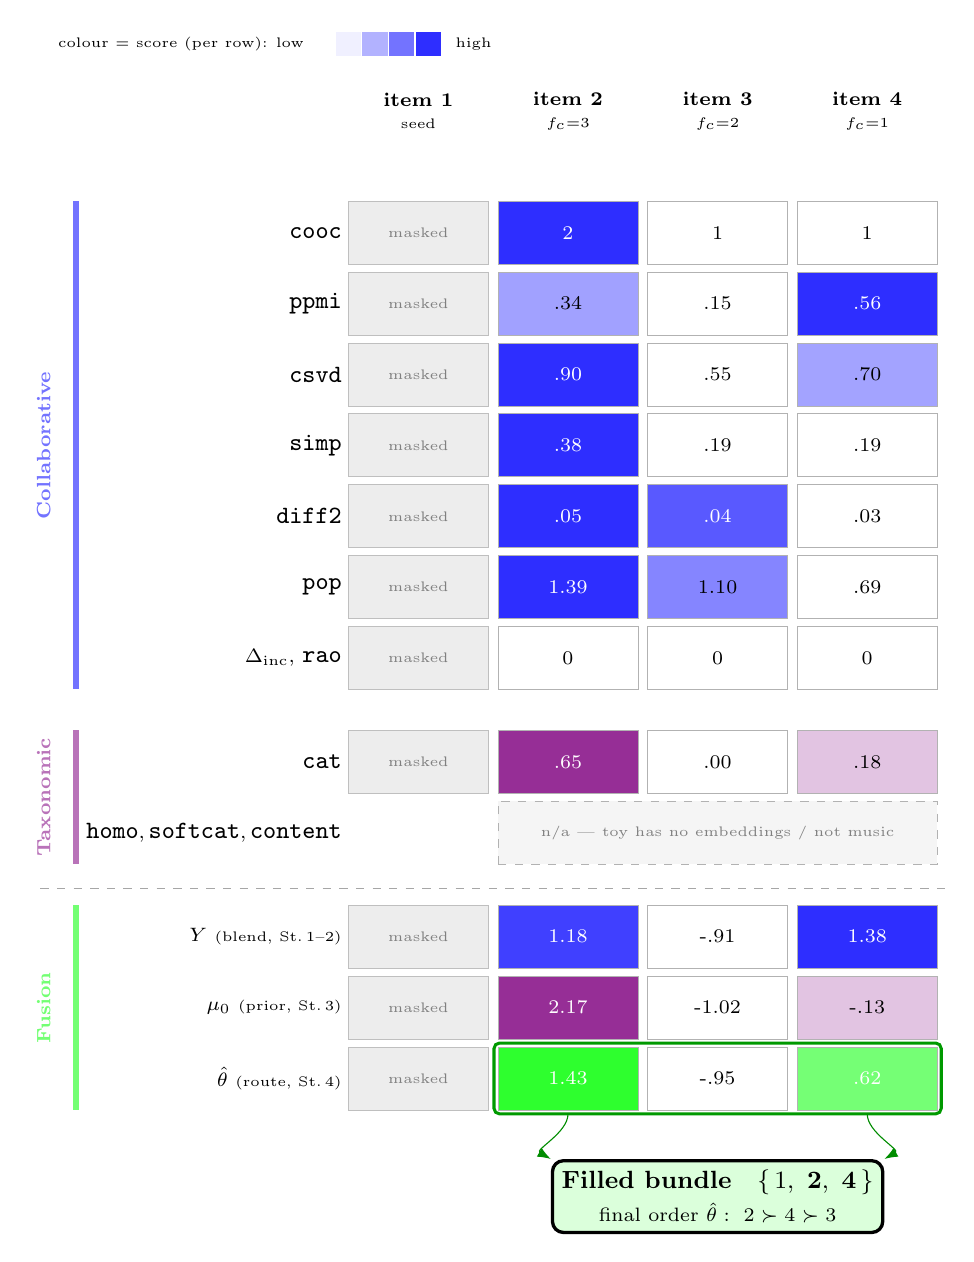
\begin{tikzpicture}[>=Latex]
% header
\node[font=\scriptsize,align=center] at (3.6,0.30){\textbf{item 1}\\{\tiny seed}};
\node[font=\scriptsize,align=center] at (5.5,0.30){\textbf{item 2}\\{\tiny $f_c{=}3$}};
\node[font=\scriptsize,align=center] at (7.4,0.30){\textbf{item 3}\\{\tiny $f_c{=}2$}};
\node[font=\scriptsize,align=center] at (9.3,0.30){\textbf{item 4}\\{\tiny $f_c{=}1$}};
\node[font=\tiny,anchor=west] at (-1.1,1.15){colour $=$ score (per row): low};
\fill[blue!6] (2.55,1.0) rectangle (2.8699999999999997,1.3);
\fill[blue!30] (2.8899999999999997,1.0) rectangle (3.2099999999999995,1.3);
\fill[blue!55] (3.23,1.0) rectangle (3.55,1.3);
\fill[blue!82] (3.57,1.0) rectangle (3.8899999999999997,1.3);
\node[font=\tiny,anchor=west] at (3.95,1.15){high};
\node[font=\scriptsize,anchor=east] at (2.75,-1.25){\code{cooc}};
\fill[black!7](2.71,-1.65) rectangle (4.49,-0.85); \draw[black!25,line width=.3pt](2.71,-1.65) rectangle (4.49,-0.85); \node[font=\tiny,gray] at (3.6,-1.25){masked};
\fill[blue!82](4.61,-1.65) rectangle (6.39,-0.85); \draw[black!30,line width=.3pt](4.61,-1.65) rectangle (6.39,-0.85); \node[font=\scriptsize,text=white] at (5.5,-1.25){2};
\fill[blue!0](6.510000000000001,-1.65) rectangle (8.290000000000001,-0.85); \draw[black!30,line width=.3pt](6.510000000000001,-1.65) rectangle (8.290000000000001,-0.85); \node[font=\scriptsize,text=black] at (7.4,-1.25){1};
\fill[blue!0](8.41,-1.65) rectangle (10.190000000000001,-0.85); \draw[black!30,line width=.3pt](8.41,-1.65) rectangle (10.190000000000001,-0.85); \node[font=\scriptsize,text=black] at (9.3,-1.25){1};
\node[font=\scriptsize,anchor=east] at (2.75,-2.15){\code{ppmi}};
\fill[black!7](2.71,-2.55) rectangle (4.49,-1.75); \draw[black!25,line width=.3pt](2.71,-2.55) rectangle (4.49,-1.75); \node[font=\tiny,gray] at (3.6,-2.15){masked};
\fill[blue!37](4.61,-2.55) rectangle (6.39,-1.75); \draw[black!30,line width=.3pt](4.61,-2.55) rectangle (6.39,-1.75); \node[font=\scriptsize,text=black] at (5.5,-2.15){.34};
\fill[blue!0](6.510000000000001,-2.55) rectangle (8.290000000000001,-1.75); \draw[black!30,line width=.3pt](6.510000000000001,-2.55) rectangle (8.290000000000001,-1.75); \node[font=\scriptsize,text=black] at (7.4,-2.15){.15};
\fill[blue!82](8.41,-2.55) rectangle (10.190000000000001,-1.75); \draw[black!30,line width=.3pt](8.41,-2.55) rectangle (10.190000000000001,-1.75); \node[font=\scriptsize,text=white] at (9.3,-2.15){.56};
\node[font=\scriptsize,anchor=east] at (2.75,-3.05){\code{csvd}};
\fill[black!7](2.71,-3.4499999999999997) rectangle (4.49,-2.65); \draw[black!25,line width=.3pt](2.71,-3.4499999999999997) rectangle (4.49,-2.65); \node[font=\tiny,gray] at (3.6,-3.05){masked};
\fill[blue!82](4.61,-3.4499999999999997) rectangle (6.39,-2.65); \draw[black!30,line width=.3pt](4.61,-3.4499999999999997) rectangle (6.39,-2.65); \node[font=\scriptsize,text=white] at (5.5,-3.05){.90};
\fill[blue!0](6.510000000000001,-3.4499999999999997) rectangle (8.290000000000001,-2.65); \draw[black!30,line width=.3pt](6.510000000000001,-3.4499999999999997) rectangle (8.290000000000001,-2.65); \node[font=\scriptsize,text=black] at (7.4,-3.05){.55};
\fill[blue!36](8.41,-3.4499999999999997) rectangle (10.190000000000001,-2.65); \draw[black!30,line width=.3pt](8.41,-3.4499999999999997) rectangle (10.190000000000001,-2.65); \node[font=\scriptsize,text=black] at (9.3,-3.05){.70};
\node[font=\scriptsize,anchor=east] at (2.75,-3.9499999999999997){\code{simp}};
\fill[black!7](2.71,-4.35) rectangle (4.49,-3.55); \draw[black!25,line width=.3pt](2.71,-4.35) rectangle (4.49,-3.55); \node[font=\tiny,gray] at (3.6,-3.9499999999999997){masked};
\fill[blue!82](4.61,-4.35) rectangle (6.39,-3.55); \draw[black!30,line width=.3pt](4.61,-4.35) rectangle (6.39,-3.55); \node[font=\scriptsize,text=white] at (5.5,-3.9499999999999997){.38};
\fill[blue!0](6.510000000000001,-4.35) rectangle (8.290000000000001,-3.55); \draw[black!30,line width=.3pt](6.510000000000001,-4.35) rectangle (8.290000000000001,-3.55); \node[font=\scriptsize,text=black] at (7.4,-3.9499999999999997){.19};
\fill[blue!0](8.41,-4.35) rectangle (10.190000000000001,-3.55); \draw[black!30,line width=.3pt](8.41,-4.35) rectangle (10.190000000000001,-3.55); \node[font=\scriptsize,text=black] at (9.3,-3.9499999999999997){.19};
\node[font=\scriptsize,anchor=east] at (2.75,-4.85){\code{diff2}};
\fill[black!7](2.71,-5.25) rectangle (4.49,-4.449999999999999); \draw[black!25,line width=.3pt](2.71,-5.25) rectangle (4.49,-4.449999999999999); \node[font=\tiny,gray] at (3.6,-4.85){masked};
\fill[blue!82](4.61,-5.25) rectangle (6.39,-4.449999999999999); \draw[black!30,line width=.3pt](4.61,-5.25) rectangle (6.39,-4.449999999999999); \node[font=\scriptsize,text=white] at (5.5,-4.85){.05};
\fill[blue!65](6.510000000000001,-5.25) rectangle (8.290000000000001,-4.449999999999999); \draw[black!30,line width=.3pt](6.510000000000001,-5.25) rectangle (8.290000000000001,-4.449999999999999); \node[font=\scriptsize,text=white] at (7.4,-4.85){.04};
\fill[blue!0](8.41,-5.25) rectangle (10.190000000000001,-4.449999999999999); \draw[black!30,line width=.3pt](8.41,-5.25) rectangle (10.190000000000001,-4.449999999999999); \node[font=\scriptsize,text=black] at (9.3,-4.85){.03};
\node[font=\scriptsize,anchor=east] at (2.75,-5.75){\code{pop}};
\fill[black!7](2.71,-6.15) rectangle (4.49,-5.35); \draw[black!25,line width=.3pt](2.71,-6.15) rectangle (4.49,-5.35); \node[font=\tiny,gray] at (3.6,-5.75){masked};
\fill[blue!82](4.61,-6.15) rectangle (6.39,-5.35); \draw[black!30,line width=.3pt](4.61,-6.15) rectangle (6.39,-5.35); \node[font=\scriptsize,text=white] at (5.5,-5.75){1.39};
\fill[blue!48](6.510000000000001,-6.15) rectangle (8.290000000000001,-5.35); \draw[black!30,line width=.3pt](6.510000000000001,-6.15) rectangle (8.290000000000001,-5.35); \node[font=\scriptsize,text=black] at (7.4,-5.75){1.10};
\fill[blue!0](8.41,-6.15) rectangle (10.190000000000001,-5.35); \draw[black!30,line width=.3pt](8.41,-6.15) rectangle (10.190000000000001,-5.35); \node[font=\scriptsize,text=black] at (9.3,-5.75){.69};
\node[font=\scriptsize,anchor=east] at (2.75,-6.65){$\Delta_{\mathrm{inc}}$, \code{rao}};
\fill[black!7](2.71,-7.050000000000001) rectangle (4.49,-6.25); \draw[black!25,line width=.3pt](2.71,-7.050000000000001) rectangle (4.49,-6.25); \node[font=\tiny,gray] at (3.6,-6.65){masked};
\fill[blue!0](4.61,-7.050000000000001) rectangle (6.39,-6.25); \draw[black!30,line width=.3pt](4.61,-7.050000000000001) rectangle (6.39,-6.25); \node[font=\scriptsize,text=black] at (5.5,-6.65){0};
\fill[blue!0](6.510000000000001,-7.050000000000001) rectangle (8.290000000000001,-6.25); \draw[black!30,line width=.3pt](6.510000000000001,-7.050000000000001) rectangle (8.290000000000001,-6.25); \node[font=\scriptsize,text=black] at (7.4,-6.65){0};
\fill[blue!0](8.41,-7.050000000000001) rectangle (10.190000000000001,-6.25); \draw[black!30,line width=.3pt](8.41,-7.050000000000001) rectangle (10.190000000000001,-6.25); \node[font=\scriptsize,text=black] at (9.3,-6.65){0};
\node[font=\scriptsize,anchor=east] at (2.75,-7.970000000000001){\code{cat}};
\fill[black!7](2.71,-8.370000000000001) rectangle (4.49,-7.57); \draw[black!25,line width=.3pt](2.71,-8.370000000000001) rectangle (4.49,-7.57); \node[font=\tiny,gray] at (3.6,-7.970000000000001){masked};
\fill[violet!82](4.61,-8.370000000000001) rectangle (6.39,-7.57); \draw[black!30,line width=.3pt](4.61,-8.370000000000001) rectangle (6.39,-7.57); \node[font=\scriptsize,text=white] at (5.5,-7.970000000000001){.65};
\fill[violet!0](6.510000000000001,-8.370000000000001) rectangle (8.290000000000001,-7.57); \draw[black!30,line width=.3pt](6.510000000000001,-8.370000000000001) rectangle (8.290000000000001,-7.57); \node[font=\scriptsize,text=black] at (7.4,-7.970000000000001){.00};
\fill[violet!23](8.41,-8.370000000000001) rectangle (10.190000000000001,-7.57); \draw[black!30,line width=.3pt](8.41,-8.370000000000001) rectangle (10.190000000000001,-7.57); \node[font=\scriptsize,text=black] at (9.3,-7.970000000000001){.18};
\node[font=\scriptsize,anchor=east] at (2.75,-8.870000000000001){\code{homo},\,\code{softcat},\,\code{content}};
\fill[black!4](4.61,-9.270000000000001) rectangle (10.190000000000001,-8.47);
\draw[black!30,dashed,line width=.3pt](4.61,-9.270000000000001) rectangle (10.190000000000001,-8.47);
\node[font=\tiny,gray] at (7.4,-8.870000000000001){n/a --- toy has no embeddings / not music};
\node[font=\scriptsize,anchor=east] at (2.75,-10.190000000000001){$Y$  {\tiny(blend, St.\,1--2)}};
\fill[black!7](2.71,-10.590000000000002) rectangle (4.49,-9.790000000000001); \draw[black!25,line width=.3pt](2.71,-10.590000000000002) rectangle (4.49,-9.790000000000001); \node[font=\tiny,gray] at (3.6,-10.190000000000001){masked};
\fill[blue!75](4.61,-10.590000000000002) rectangle (6.39,-9.790000000000001); \draw[black!30,line width=.3pt](4.61,-10.590000000000002) rectangle (6.39,-9.790000000000001); \node[font=\scriptsize,text=white] at (5.5,-10.190000000000001){1.18};
\fill[blue!0](6.510000000000001,-10.590000000000002) rectangle (8.290000000000001,-9.790000000000001); \draw[black!30,line width=.3pt](6.510000000000001,-10.590000000000002) rectangle (8.290000000000001,-9.790000000000001); \node[font=\scriptsize,text=black] at (7.4,-10.190000000000001){-.91};
\fill[blue!82](8.41,-10.590000000000002) rectangle (10.190000000000001,-9.790000000000001); \draw[black!30,line width=.3pt](8.41,-10.590000000000002) rectangle (10.190000000000001,-9.790000000000001); \node[font=\scriptsize,text=white] at (9.3,-10.190000000000001){1.38};
\node[font=\scriptsize,anchor=east] at (2.75,-11.090000000000002){$\mu_0$  {\tiny(prior, St.\,3)}};
\fill[black!7](2.71,-11.490000000000002) rectangle (4.49,-10.690000000000001); \draw[black!25,line width=.3pt](2.71,-11.490000000000002) rectangle (4.49,-10.690000000000001); \node[font=\tiny,gray] at (3.6,-11.090000000000002){masked};
\fill[violet!82](4.61,-11.490000000000002) rectangle (6.39,-10.690000000000001); \draw[black!30,line width=.3pt](4.61,-11.490000000000002) rectangle (6.39,-10.690000000000001); \node[font=\scriptsize,text=white] at (5.5,-11.090000000000002){2.17};
\fill[violet!0](6.510000000000001,-11.490000000000002) rectangle (8.290000000000001,-10.690000000000001); \draw[black!30,line width=.3pt](6.510000000000001,-11.490000000000002) rectangle (8.290000000000001,-10.690000000000001); \node[font=\scriptsize,text=black] at (7.4,-11.090000000000002){-1.02};
\fill[violet!23](8.41,-11.490000000000002) rectangle (10.190000000000001,-10.690000000000001); \draw[black!30,line width=.3pt](8.41,-11.490000000000002) rectangle (10.190000000000001,-10.690000000000001); \node[font=\scriptsize,text=black] at (9.3,-11.090000000000002){-.13};
\node[font=\scriptsize,anchor=east] at (2.75,-11.990000000000002){$\hat\theta$  {\tiny(route, St.\,4)}};
\fill[black!7](2.71,-12.390000000000002) rectangle (4.49,-11.590000000000002); \draw[black!25,line width=.3pt](2.71,-12.390000000000002) rectangle (4.49,-11.590000000000002); \node[font=\tiny,gray] at (3.6,-11.990000000000002){masked};
\fill[green!82](4.61,-12.390000000000002) rectangle (6.39,-11.590000000000002); \draw[black!30,line width=.3pt](4.61,-12.390000000000002) rectangle (6.39,-11.590000000000002); \node[font=\scriptsize,text=white] at (5.5,-11.990000000000002){1.43};
\fill[green!0](6.510000000000001,-12.390000000000002) rectangle (8.290000000000001,-11.590000000000002); \draw[black!30,line width=.3pt](6.510000000000001,-12.390000000000002) rectangle (8.290000000000001,-11.590000000000002); \node[font=\scriptsize,text=black] at (7.4,-11.990000000000002){-.95};
\fill[green!54](8.41,-12.390000000000002) rectangle (10.190000000000001,-11.590000000000002); \draw[black!30,line width=.3pt](8.41,-12.390000000000002) rectangle (10.190000000000001,-11.590000000000002); \node[font=\scriptsize,text=white] at (9.3,-11.990000000000002){.62};
\draw[blue!55,line width=2pt](-0.75,-0.85) -- (-0.75,-7.050000000000001);
\node[font=\scriptsize\bfseries,rotate=90,anchor=south,text=blue!55] at (-0.95,-3.95){Collaborative};
\draw[violet!55,line width=2pt](-0.75,-7.57) -- (-0.75,-9.270000000000001);
\node[font=\scriptsize\bfseries,rotate=90,anchor=south,text=violet!55] at (-0.95,-8.420000000000002){Taxonomic};
\draw[green!55,line width=2pt](-0.75,-9.790000000000001) -- (-0.75,-12.390000000000002);
\node[font=\scriptsize\bfseries,rotate=90,anchor=south,text=green!55] at (-0.95,-11.090000000000002){Fusion};
\draw[black!35,dashed](-1.2,-9.58) -- (10.290000000000001,-9.58);
\draw[green!60!black,line width=1.1pt,rounded corners=2pt](4.5600000000000005,-12.440000000000003) rectangle (10.240000000000002,-11.540000000000001);
\node[draw,very thick,rounded corners,fill=green!14,font=\small,align=center] (OUT) at (7.4,-13.490000000000002){\textbf{Filled bundle}\quad $\{\,1,\ \mathbf{2},\ \mathbf{4}\,\}$\\[1pt]{\scriptsize final order $\hat\theta:\ 2\succ4\succ3$}};
\draw[->,green!55!black](5.5,-12.440000000000003) to[out=-90,in=150] (OUT.north west);
\draw[->,green!55!black](9.3,-12.440000000000003) to[out=-90,in=30] (OUT.north east);
\end{tikzpicture}
\end{center}
\captionof{figure}{\textbf{How a partial bundle is filled, as a score map.} Columns are catalogue items, rows are the
method's signals grouped by family; each cell is that signal's score for that item, \emph{shaded darker when higher}
(normalised within the row), with the exact toy number inside. The seed item~$1$ is \emph{masked} (never scored). Read
it top-to-bottom: the \textbf{collaborative} signals score by (co-)occurrence---note they mostly favour the hub
item~$2$, except \code{ppmi}, which backs the rare item~$4$; the \textbf{taxonomic} \code{cat} favours item~$2$
(category $A$ complements $B$); \code{homo}/\code{softcat}/\code{content} are \emph{n/a} here because the toy has no
embeddings/music (shown, not hidden); the set-level $\Delta_{\mathrm{inc}}$/\code{rao} are $0$ (a single seed forms no
pair). The \textbf{fusion} band then collapses every row into one score per item: the validation-weighted blend $Y$
(Stages 1--2), the cold-start prior $\mu_0$ (Stage 3), and their per-item mix $\hat\theta=(1-u_c)Y+u_c\mu_0$ with
$u_c=\kappa/(f_c+\kappa)$ (Stage 4). Ranking $\hat\theta$ (highlighted) and dropping the seed yields the completion
$\{1,\mathbf2,\mathbf4\}$. Every number is machine-verified; the same $\hat\theta$ appears in Fig.~\ref{fig:stages}.}
\label{fig:flow}

The note is bottom-up. \S\ref{sec:inputs}--\S\ref{sec:derived} define what we start with. \S\ref{sec:vocab} defines
the five recurring \emph{operations} (co-occurrence, PMI, SVD, degree normalisation, graph propagation) precisely as
used here. \S\ref{sec:signals} builds every individual \emph{signal} from those operations. \S\ref{sec:toscore}
turns a signal into per-query numbers. \S\ref{sec:fuse} is the four-stage fusion that produces the final score.
\S\ref{sec:ledger} is the ledger of what is learned versus fixed.

\begin{keybox}
\textbf{The running toy dataset (used in every example).} Catalogue of $n=4$ items $\{1,2,3,4\}$ and three
training bundles
\[
  b_1=\{1,2,3\},\qquad b_2=\{1,2,4\},\qquad b_3=\{2,3\}.
\]
\end{keybox}

% ======================================================================
\section{What we start with: the raw inputs}
\label{sec:inputs}

\subsection{The items, the bundles, and the incidence matrix}

The \textbf{catalogue} is a finite set of items $\I=\{1,\dots,n\}$. The \textbf{training data} is a collection of
$m$ bundles $\B=\{b_1,\dots,b_m\}$, each a subset of items. We record them once in a \textbf{bundle--item incidence
matrix}
\[
  B\in\{0,1\}^{m\times n},\qquad B_{ji}=\begin{cases}1 & \text{item $i$ is in bundle $j$}\\ 0 &\text{otherwise.}\end{cases}
\]
Every bundle is a \emph{row}; every item is a \emph{column}. This single matrix is the backbone of every
collaborative signal. (In code: \code{SimplicialGraphOperator} builds \code{self.B} and its binary version
\code{self.B\_bin}.)

\begin{example}[the incidence matrix]\label{ex:B}
For the toy dataset,
\[
  B=\begin{pmatrix}1&1&1&0\\ 1&1&0&1\\ 0&1&1&0\end{pmatrix}
  \begin{array}{l}\leftarrow b_1=\{1,2,3\}\\ \leftarrow b_2=\{1,2,4\}\\ \leftarrow b_3=\{2,3\}\end{array}
\]
\end{example}

\begin{center}
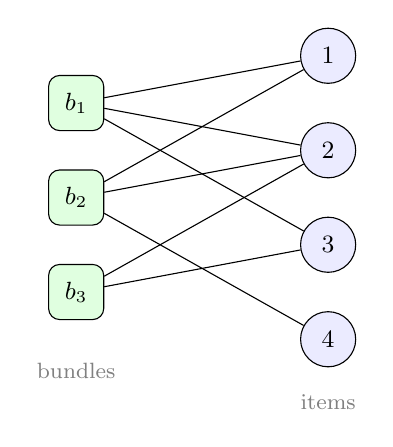
\begin{tikzpicture}[>=Latex,
  item/.style={circle,draw,minimum size=7mm,inner sep=0pt,fill=blue!8,font=\small},
  bun/.style={rectangle,draw,rounded corners,minimum size=7mm,fill=green!12,font=\small}]
  \node[bun] (b1) at (0,1.8)  {$b_1$};
  \node[bun] (b2) at (0,0.6)  {$b_2$};
  \node[bun] (b3) at (0,-0.6) {$b_3$};
  \node[item] (i1) at (3.2,2.4)  {1};
  \node[item] (i2) at (3.2,1.2)  {2};
  \node[item] (i3) at (3.2,0.0)  {3};
  \node[item] (i4) at (3.2,-1.2) {4};
  \draw (b1)--(i1); \draw (b1)--(i2); \draw (b1)--(i3);
  \draw (b2)--(i1); \draw (b2)--(i2); \draw (b2)--(i4);
  \draw (b3)--(i2); \draw (b3)--(i3);
  \node[font=\footnotesize,gray] at (0,-1.6)  {bundles};
  \node[font=\footnotesize,gray] at (3.2,-2.0) {items};
\end{tikzpicture}
\end{center}
\captionof{figure}{\emph{The bundle--item graph of the toy data.} Each edge is a $1$ in $B$. The \textbf{degree of an item}
(number of edges) is its frequency $f$: item $2$ has $3$ edges ($f_2=3$), item $4$ has one ($f_4=1$). Two items
\textbf{co-occur} ($C_{ci}>0$) exactly when they connect to a common bundle box: items $1$ and $2$ share $b_1$ and
$b_2$ (so $C_{12}=2$), while items $3$ and $4$ share no box ($C_{34}=0$). Every collaborative signal in this note is
some way of reading this one picture.}
\label{fig:graph}

\subsection{The embedding features --- stated explicitly}
\label{sec:emb}

Besides the bundles, each item carries \textbf{pretrained embedding vectors}: fixed real-valued feature vectors that
describe the item's \emph{content} (what it looks like, what it is called, what it sounds like). \textbf{\textsc{BundleFuse}
does not train these. It loads them from the public dataset release and treats them as constants.} They enter only
the \emph{content} and \emph{soft-category} signals (\S\ref{sec:content},\,\S\ref{sec:tax}); the collaborative and
taxonomic signals never touch them. The exact tensors (read in \code{fullrank\_eval.py}, lines 118--133) are:

\begin{center}\small
\begin{tabular}{@{}l l l l@{}}
\toprule
File on disk & Role in code & Shape (e.g.\ \textsc{POG}) & What it is \\
\midrule
\code{title\_emb.npy} & \code{feats["content"]} & $48676\times 512$ & text embedding of the item \emph{title} \\
\code{content\_feature.pt} & \code{feats["image"]} (fashion) & $48676\times 768$ & \emph{image} embedding of the product photo \\
                           & \code{feats["audio"]} (music) & $254155\times 512$ & \emph{audio} embedding of the track \\
\code{description\_feature.pt} & \code{feats["desc"]} & $48676\times 768$ & text embedding of the \emph{description} \\
\bottomrule
\end{tabular}
\end{center}

\paragraph{Where every vector comes from (so no number is unexplained).} There are two distinct sources, and we name
both.
\emph{(i) Image / description / audio --- from the public release.} \code{content\_feature.pt} and
\code{description\_feature.pt} are the pre-extracted features shipped with the public \textsc{BundleConstruction}
release (Liu et al., \emph{Fine-tuning Multimodal LLMs for Product Bundling / Bundle-MLLM}, KDD 2025) and consumed
unchanged --- the same features the heavy baselines use. Their origin is documented in the \textbf{CLHE} paper
(Ma et al., ``Leveraging Multimodal Features and Item-level User Feedback for Bundle Construction,'' WSDM 2024;
\code{arXiv:2310.18770}), whose dataset the \textsc{BundleConstruction} release \emph{is}, and corroborated by RaMen
(ECAI 2025, \S3.1.2): for \textsc{POG} the visual and textual vectors are produced by \textbf{pre-trained BLIP}
(Li et al., ``BLIP: Bootstrapping Language-Image Pre-training,'' ICML 2022), hence their $768$ dimensions; for
\textsc{Spotify} the audio vector is produced by \textbf{CLAP} (Wu et al., ``Large-scale Contrastive
Language--Audio Pretraining,'' 2023), which is why Spotify's content vector is $512$-d (CLAP's native embedding size)
rather than $768$-d. The release \emph{also} ships LightGCN collaborative features (\code{item\_cf\_feature.pt},
\code{*\_LightGCN\_bi\_feature.pt}), which we deliberately do \textbf{not} load --- reusing precomputed collaborative
features under our re-split would leak held-out co-occurrence (it once manufactured a $16\times$ phantom win on
\textsc{POG}); we rebuild every collaborative signal from the train fold instead.
\emph{(ii) Title --- generated by us.} \code{title\_emb.npy} ($48676\times512$) is \textbf{not} from the release and
\textbf{not} a mystery: \emph{we} produce it with the script \code{embed\_titles.py}, which runs a frozen
\textbf{\code{BAAI/bge-small-zh-v1.5}} Chinese sentence-encoder (via \code{sentence\_transformers},
\code{normalize\_embeddings=True}) over the \textsc{POG} item titles --- which are in Chinese, since \textsc{POG} is
Alibaba iFashion. Its $512$ dimensions are exactly that model's hidden size; the companion \code{title\_emb\_large.npy}
($1024$-d) is the identical script with \code{BAAI/bge-large-zh-v1.5}. So every content input is now sourced: BLIP
(release, via CLHE) for \textsc{POG} image/description, CLAP (release, via CLHE) for \textsc{Spotify} audio, and a
frozen BGE encoder (ours) for the \textsc{POG} titles.

\noindent Every vector is \textbf{$L_2$-normalised} on load (\code{\_loadpt}: $x\leftarrow x/\lVert x\rVert_2$), so a
dot product between two of them is a cosine similarity in $[-1,1]$. For \textsc{POG} the three are concatenated into
a single $512{+}768{+}768=2048$-dimensional multimodal vector (\code{mm\_feat}) used for clustering; for music only
the $512$-d audio vector exists (the code detects this via the \emph{absence} of \code{title\_emb.npy} and sets the
internal \code{MUSIC} flag).

\paragraph{Not every dataset uses an external encoder.} The table above is for \textsc{POG} and \textsc{Spotify}
only. On the e-commerce sets (\textsc{Electronic}/\textsc{Food}/\textsc{Clothing}) and the grocery set
(\textsc{Dunnhumby}) there is \textbf{no pretrained embedding at all}: the content signal is a plain \textbf{TF--IDF}
vector of the item's own text fields (department / commodity / brand / title), reduced by truncated SVD, computed
\emph{inside} the pipeline (\code{bundlerec\_eval.py}:106; \code{dunnhumby\_eval.py}:80--83). So ``content'' means two
different things depending on the dataset --- a deep BLIP/CLIP embedding on POG/Spotify, a classical bag-of-words
vector on the e-commerce/grocery sets --- and we say so plainly rather than imply one uniform source. \textbf{If a
dataset ships neither, the content signals are simply absent and the method runs on collaborative$+$taxonomic
evidence alone.}

\paragraph{Deployment consequence.} Because the POG/Spotify content signals are \emph{functions of these encoders'
outputs}, serving the method on a genuinely new item requires first running the same encoders (BLIP on the item's
image and description and BGE on its title for fashion, or CLAP on the track for music) to embed it, before any
content/soft-category signal can place it. The TF--IDF datasets need
no external model --- only the item's text. We state this so the true dependency footprint is explicit: the
``zero-parameter'' claim is about the \emph{scorer} (it fits no weights by gradient descent), not about these upstream
feature extractors, which are a real deployment prerequisite wherever deep content features are used.

\subsection{The side labels: categories, artists, albums}

Each item also has discrete \textbf{metadata labels}. For fashion that is an explicit category id \code{cate}
(e.g.\ ``boots''); for music it is the \code{artist\_uri} and \code{album\_uri}. We store them as integer label
vectors $\mathrm{cat}\in\{0,\dots,C-1\}^n$ (and, for music, $\mathrm{alb}$). When a dataset has \emph{no} usable
category, the code manufactures one by running $k$-means ($400$ clusters) on the multimodal embedding and using the
cluster id as a pseudo-category (\code{fullrank\_eval.py}:146--156). These labels feed the \emph{taxonomic} signals
(\S\ref{sec:tax}).

% ======================================================================
\section{Three structures we derive immediately}
\label{sec:derived}

Everything collaborative is built from three quantities read straight off $B$.

\paragraph{(1) Item frequency $f$.} How many training bundles contain each item:
\[
  f=B^{\!\top}\onevec_m\in\mathbb{Z}^n,\qquad f_i=\#\{\text{bundles containing }i\}.
\]
An item with $f_i=0$ is \textbf{cold} (never seen in training); cold items are exactly where the collaborative
signals go silent and the prior has to take over (\S\ref{sec:fuse}). In code: \code{self.freq = B.sum(0)}.

\paragraph{(2) Co-occurrence matrix $C$.} How often each \emph{pair} of items shares a bundle, with the diagonal
removed (we never ``co-occur'' an item with itself):
\[
  C=B^{\!\top}B,\qquad C_{ii}\leftarrow 0 .
\]
$C_{ci}$ = number of training bundles containing both $c$ and $i$. In code: \code{self.C = (B.T @ B)} then
\code{C.setdiag(0)}.

\paragraph{(3) Bundle sizes.} $|b_j|=\sum_i B_{ji}$, used to down-weight large bundles (a pair that co-occurs inside
a $20$-item playlist is weaker evidence than a pair that co-occurs inside a $2$-item set). In code: \code{self.bsize}.

\begin{example}[the three structures]\label{ex:derived}
From $B$ in Example~\ref{ex:B}:
\[
  f=\begin{pmatrix}2\\3\\2\\1\end{pmatrix},\qquad
  B^{\!\top}B=\begin{pmatrix}2&2&1&1\\2&3&2&1\\1&2&2&0\\1&1&0&1\end{pmatrix}
  \;\xrightarrow{\text{zero diag}}\;
  C=\begin{pmatrix}0&2&1&1\\2&0&2&1\\1&2&0&0\\1&1&0&0\end{pmatrix}.
\]
Read $C$ as: items $1$ and $2$ share $2$ bundles; items $3$ and $4$ never share one. Item $2$ is the most frequent
($f_2=3$); item $4$ the rarest ($f_4=1$).
\end{example}

\begin{center}
\resizebox{\linewidth}{!}{%
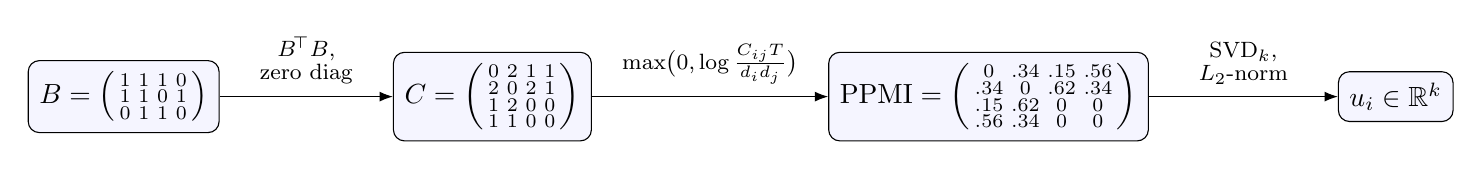
\begin{tikzpicture}[>=Latex,
  mat/.style={draw,rounded corners,fill=blue!4,inner sep=4pt},
  lbl/.style={font=\footnotesize,align=center,midway,above,yshift=1pt}]
\node[mat] (B) {$B=\left(\begin{smallmatrix}1&1&1&0\\1&1&0&1\\0&1&1&0\end{smallmatrix}\right)$};
\node[mat,right=22mm of B] (C) {$C=\left(\begin{smallmatrix}0&2&1&1\\2&0&2&1\\1&2&0&0\\1&1&0&0\end{smallmatrix}\right)$};
\node[mat,right=30mm of C] (P) {$\mathrm{PPMI}=\left(\begin{smallmatrix}0&.34&.15&.56\\.34&0&.62&.34\\.15&.62&0&0\\.56&.34&0&0\end{smallmatrix}\right)$};
\node[mat,right=24mm of P] (U) {$u_i\in\R^{k}$};
\draw[->](B)--(C) node[lbl]{$B^{\!\top}B$,\\[-1pt]zero diag};
\draw[->](C)--(P) node[lbl]{$\max\!\big(0,\log\tfrac{C_{ij}T}{d_id_j}\big)$};
\draw[->](P)--(U) node[lbl]{SVD$_k$,\\[-1pt]$L_2$-norm};
\end{tikzpicture}}
\end{center}
\captionof{figure}{\emph{The collaborative pipeline, built once from the bundles alone.} The bundle--item matrix $B$ becomes the
item--item co-occurrence $C=B^{\!\top}B$ (diagonal zeroed); $C$ becomes the chance-corrected $\mathrm{PPMI}$
(\S\ref{sec:pmi}); and a truncated SVD of $\mathrm{PPMI}$ gives each item a dense ``collaborative fingerprint'' $u_i$
(\S\ref{sec:svd}). The partial bundle is \emph{not} involved yet: these are fixed structures a query is later scored
\emph{against}.}
\label{fig:build}

% ======================================================================
\section{The vocabulary of operations (general idea $\to$ local definition $\to$ example)}
\label{sec:vocab}

Five operations recur throughout. Each is a standard idea, but what matters is \emph{the exact quantity it is
applied to here}. This section pins that down; \S\ref{sec:signals} then just assembles them.

\subsection{Co-occurrence scoring: ``who shows up with the seeds''}

\paragraph{General.} The simplest bundle signal: score a candidate $c$ by how often it co-occurred with the seed
items. If $\xs\in\{0,1\}^n$ is the \textbf{seed indicator} ($(\xs)_i=1$ iff $i\in S$), then
\[
  \text{cooc}(c\mid S)=\sum_{i\in S}C_{ci}=(C\,\xs)_c .
\]
A matrix--vector product: the score vector is column-combination of $C$ selected by the seeds.

\paragraph{Here.} Exactly this, with $C$ the zero-diagonal co-occurrence matrix above. In code the seed indicators
for a whole batch of queries are stacked into a sparse matrix \code{Ind} ($n\times\text{nb}$, one column per query)
and the batch of score vectors is the single product \code{C @ Ind} (\code{fullrank\_eval.py}:262). This
``$W\,\xs$'' shape is the template for \emph{every} collaborative signal.

\begin{example}[co-occurrence scores]\label{ex:cooc}
Query $S=\{1\}$, so $\xs=(1,0,0,0)^{\!\top}$ and $C\xs$ is column $1$ of $C$:
\[
  C\xs=(0,\,2,\,1,\,1)^{\!\top}.
\]
Excluding the seed, the ranking is $2\succ 3\!\sim\!4$: item $2$ (shared $2$ bundles with item $1$) wins. Hold this
result---PMI will \emph{overturn} it.
\end{example}

\begin{center}
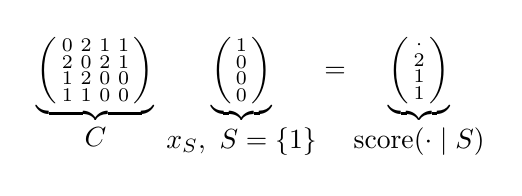
\begin{tikzpicture}[>=Latex]
\node (eq) {$\underbrace{\left(\begin{smallmatrix}0&2&1&1\\2&0&2&1\\1&2&0&0\\1&1&0&0\end{smallmatrix}\right)}_{\textstyle C}\;
\underbrace{\left(\begin{smallmatrix}1\\0\\0\\0\end{smallmatrix}\right)}_{\textstyle x_S,\ S=\{1\}}
=\underbrace{\left(\begin{smallmatrix}\cdot\\2\\1\\1\end{smallmatrix}\right)}_{\textstyle \mathrm{score}(\cdot\mid S)}$};
\end{tikzpicture}
\end{center}
\captionof{figure}{\emph{Filling a partial bundle is one matrix--vector product.} The seed indicator $x_S$ carries a $1$ in each
seed slot, so $Cx_S$ \textbf{sums the seed columns of $C$}. For $S=\{1\}$ it reads off column $1$: candidate $2$
scores $2$, candidates $3,4$ score $1$; the seed itself ($c=1$, shown ``$\cdot$'') is masked to $-\infty$ before
ranking. \emph{Every} collaborative signal has this exact shape $Wx_S$---only the matrix $W$ changes (raw $C$,
$\mathrm{PPMI}$, the degree-normalised $W_{\text{pair}}$, or the household operator).}
\label{fig:cooc}

\subsection{PMI / PPMI: ``is this pair together \emph{more than chance}?''}
\label{sec:pmi}

\paragraph{General.} Raw co-occurrence is biased toward popular items: a hub co-occurs with everything. Pointwise
Mutual Information corrects for that by comparing the \emph{joint} probability of a pair to the product of their
\emph{marginals}:
\[
  \mathrm{PMI}(i,j)=\log\frac{P(i,j)}{P(i)\,P(j)} .
\]
It is positive when $i,j$ appear together more than independence predicts, negative when less. The \emph{positive}
part, $\mathrm{PPMI}=\max(0,\mathrm{PMI})$, keeps only genuine associations (and is what makes the matrix sparse and
well-behaved for the SVD below).

\paragraph{Here --- and this is the subtle part.} The probabilities are estimated \textbf{from the co-occurrence
matrix $C$ itself}, not from item frequencies $f$. Let
\[
  d_i=\sum_{j}C_{ij}\quad(\text{row sum of }C,\ \text{the ``co-occurrence degree'' of }i),\qquad
  T=\sum_{i,j}C_{ij}\quad(\text{grand total}).
\]
Then the \emph{joint} is $P(i,j)=C_{ij}/T$ and the \emph{marginals} are $P(i)=d_i/T$, giving
\begin{keybox}
\[
  \mathrm{PPMI}_{ij}=\max\!\Big(0,\ \log\frac{C_{ij}\,T}{d_i\,d_j}\Big),\qquad
  d_i=\textstyle\sum_j C_{ij},\quad T=\sum_{i,j}C_{ij}.
\]
\end{keybox}
\textbf{Note what the ``marginal'' is here: the co-occurrence degree $d_i$ (how much total pairing mass item $i$
carries), not the bundle-frequency $f_i$.} These differ---e.g.\ a popular item in many \emph{singleton-ish} bundles
has high $f$ but modest $d$. The code (\code{operators.py}:103--107) uses precisely $d$ and $T$ derived from $C$:
\code{freq\_c = C.sum(1)}, \code{totc = C.sum()}. The same construction is reused verbatim for \emph{category}
co-occurrence and for \emph{soft-cluster} co-occurrence (\S\ref{sec:tax})---same formula, different ``vocabulary''
(items, categories, or clusters).

\begin{example}[PPMI overturns raw co-occurrence]\label{ex:ppmi}
Degrees are the row sums of $C$ from Example~\ref{ex:derived}: $d=(4,5,3,2)$, and $T=14$. Then, e.g.,
\[
  \mathrm{PMI}(1,2)=\log\frac{2\cdot 14}{4\cdot 5}=\log 1.4=0.336,\qquad
  \mathrm{PMI}(1,4)=\log\frac{1\cdot 14}{4\cdot 2}=\log 1.75=0.560 .
\]
The full positive matrix is
\[
  \mathrm{PPMI}=\begin{pmatrix}0&0.336&0.154&0.560\\ 0.336&0&0.624&0.336\\
  0.154&0.624&0&0\\ 0.560&0.336&0&0\end{pmatrix}.
\]
Now re-score query $S=\{1\}$ (column $1$): $(0,\,0.336,\,0.154,\,0.560)$, ranking
\[
  \boxed{4\ \succ\ 2\ \succ\ 3}\qquad\text{(was }2\succ3\!\sim\!4\text{ under raw co-occurrence).}
\]
\textbf{Item $4$ jumped to first.} Why: item $4$ is rare ($d_4=2$), so its single shared bundle with item $1$ is
``surprising'' and informative, whereas item $2$ is a hub ($d_2=5$) that pairs with everyone, so sharing two
bundles with it is partly explained by chance. That reweighting is the entire point of PMI, and it is why we keep a
PPMI channel alongside raw co-occurrence.
\end{example}

\begin{center}
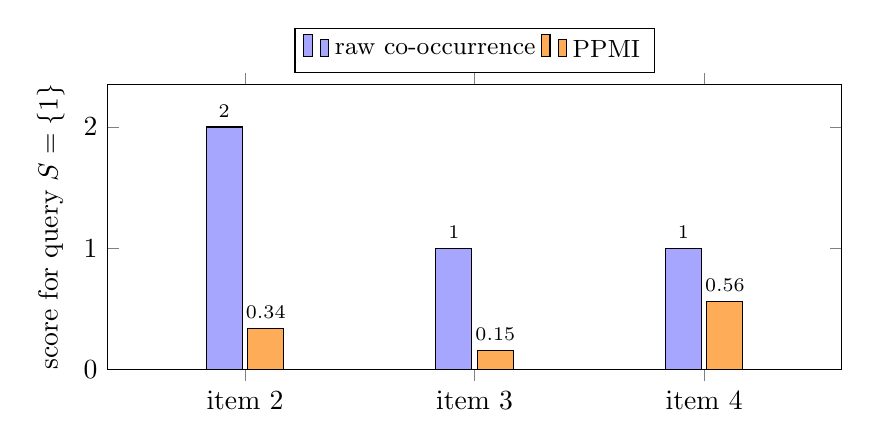
\begin{tikzpicture}
\begin{axis}[ybar,bar width=13pt,width=0.9\linewidth,height=5.2cm,
  symbolic x coords={item 2,item 3,item 4},xtick=data,
  ymin=0,ymax=2.35,enlarge x limits=0.3,
  ylabel={score for query $S=\{1\}$},
  legend style={font=\small,at={(0.5,1.04)},anchor=south,legend columns=2},
  nodes near coords,every node near coord/.append style={font=\scriptsize}]
\addplot[fill=blue!35] coordinates {(item 2,2) (item 3,1) (item 4,1)};
\addplot[fill=orange!65] coordinates {(item 2,0.336) (item 3,0.154) (item 4,0.560)};
\legend{raw co-occurrence,PPMI}
\end{axis}
\end{tikzpicture}
\end{center}
\captionof{figure}{\emph{Same query, two signals, opposite winners.} Raw co-occurrence (blue) crowns the \emph{hub} item $2$;
PPMI (orange), by dividing out each item's popularity, crowns the \emph{rare-but-exclusive} item $4$. The PPMI bars
are shorter in absolute terms (they are log-ratios), but standardisation in \S\ref{sec:toscore} removes that scale
difference---what survives into the blend is the \emph{ordering}.}
\label{fig:ppmi}

\subsection{Truncated SVD: a dense ``collaborative fingerprint'' per item}
\label{sec:svd}

\paragraph{General.} A truncated singular value decomposition approximates a matrix by the best rank-$k$ product
$M\approx U\Sigma V^{\!\top}$; the rows of $U\Sigma$ (here we keep $U$) are a $k$-dimensional \emph{embedding} of the
objects, capturing their dominant patterns of variation while discarding noise.

\paragraph{Here.} The SVD is taken of the \textbf{item--item PPMI matrix}, \emph{not} of a user--item rating matrix.
With $k=128$ (\code{TruncatedSVD(n\_components=128)} on \code{self.PPMI}, \code{operators.py}:108--111), we get a
$128$-dimensional vector per item and $L_2$-normalise each row:
\[
  U=\mathrm{SVD}_{128}(\mathrm{PPMI}),\qquad u_i=U_i/\lVert U_i\rVert_2 .
\]
Think of $u_i$ as item $i$'s ``collaborative fingerprint'': two items get similar fingerprints when they pair with
\emph{similar sets of partners}, even if they never co-occur \emph{directly}. This is the only embedding the method
builds itself, and it is built from co-occurrence alone---no external features. It is stored as \code{self.Ucsvd}
and exposed as the signal \code{csvd}.

\begin{remark}[direct vs.\ indirect association]
Raw co-occurrence and PPMI see only \emph{direct} pairs ($C_{ci}>0$). The SVD fingerprint sees \emph{second-order}
structure: items $3$ and $4$ never co-occur ($C_{34}=0$), yet both co-occur with $\{1,2\}$, so their fingerprints are
pulled closer. This is how the collaborative side reasons about pairs it has never literally observed together.
\end{remark}

\begin{center}
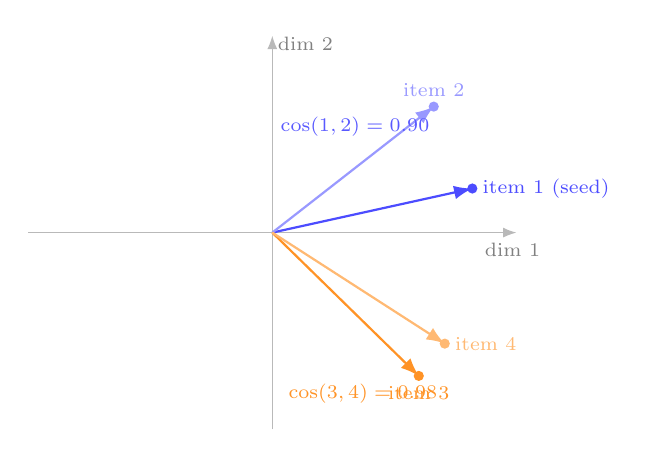
\begin{tikzpicture}[>=Latex,dot/.style={circle,fill,inner sep=1.3pt}]
\draw[->,gray!55](-3.1,0)--(3.1,0); \draw[->,gray!55](0,-2.5)--(0,2.5);
\node[font=\scriptsize,gray] at (3.05,-0.22){dim 1}; \node[font=\scriptsize,gray] at (0.42,2.4){dim 2};
\draw[->,thick,blue!70](0,0)--(2.54,0.56) node[dot]{} node[right,font=\scriptsize]{item $1$ (seed)};
\draw[->,thick,blue!40](0,0)--(2.05,1.60) node[dot]{} node[above,font=\scriptsize]{item $2$};
\draw[->,thick,orange!85](0,0)--(1.86,-1.82) node[dot]{} node[below,font=\scriptsize]{item $3$};
\draw[->,thick,orange!55](0,0)--(2.19,-1.41) node[dot]{} node[right,font=\scriptsize]{item $4$};
\node[font=\scriptsize,orange!85] at (1.15,-2.05){$\cos(3,4)=0.98$};
\node[font=\scriptsize,blue!65] at (1.05,1.35){$\cos(1,2)=0.90$};
\end{tikzpicture}
\end{center}
\captionof{figure}{\emph{The fingerprint sees partners-of-partners, not just direct pairs.} These are the \textbf{exact} rank-$2$
$L_2$-normalised fingerprints $u_i$ of the toy $\mathrm{PPMI}$ (machine-computed, $x$-sign flipped for display). Items
$3$ and $4$ \textbf{never co-occur} ($C_{34}=0$), yet their fingerprints are almost identical ($\cos=0.98$) because
both pair with $\{1,2\}$; the hubs $1,2$ likewise sit together ($\cos=0.90$). The \code{csvd} score of a candidate is
the cosine between its fingerprint and the seeds' \emph{average} fingerprint---so a partial bundle recalls items with
the same \emph{company}, even ones never literally seen with it.}
\label{fig:fingerprint}

\subsection{Degree normalisation: taming hubs and big bundles}
\label{sec:degnorm}

\paragraph{General.} Popular items and large bundles dominate raw sums. We damp them with two monotone discounts.

\paragraph{Here.} Two fixed vectors (\code{operators.py}:79--81), with smoothing constants read directly from code:
\[
  \underbrace{(f_i+5)^{-0.5}}_{\text{item discount}}\qquad\text{and}\qquad \underbrace{(|b|+1)^{-0.5}}_{\text{bundle-size discount}} .
\]
The ``$+5$'' and ``$+1$'' are smoothing (they stop rare items/small bundles from blowing up); the exponent $0.5$ is a
square-root taming. These assemble into the \textbf{degree-normalised pairwise operator}
\begin{keybox}
\[
  W_{\text{pair}} \;=\; B^{\!\top}\,\mathrm{diag}\!\big((|b|+1)^{-0.5}\big)\,B\,\mathrm{diag}\!\big((f+5)^{-0.5}\big),
  \qquad \mathrm{diag}(W_{\text{pair}})=0 .
\]
\end{keybox}
Reading it right-to-left: scale each seed column by its item discount, walk bundle$\to$items weighting each bundle by
its size discount, land back on items. So $W_{\text{pair}}(c\mid S)=\sum_{b\ni c}(|b|+1)^{-0.5}\sum_{s\in S\cap
b}(f_s+5)^{-0.5}$: a \emph{smoothed, size-aware} co-occurrence. Setting both exponents to $0$ recovers plain $C$
(the case used in Examples~\ref{ex:cooc}--\ref{ex:ppmi} for clarity).

\begin{center}
\resizebox{\linewidth}{!}{%
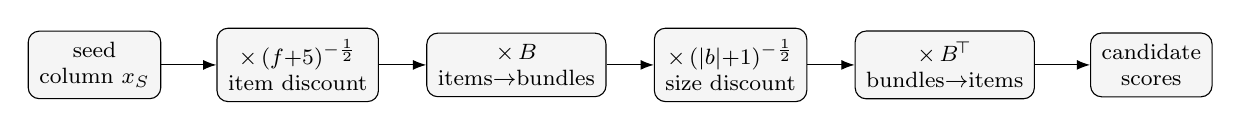
\begin{tikzpicture}[>=Latex,
  bl/.style={draw,rounded corners,fill=black!4,inner sep=4pt,font=\footnotesize,align=center}]
\node[bl](x){seed\\column $x_S$};
\node[bl,right=7mm of x](d1){$\times\,(f{+}5)^{-\frac12}$\\item discount};
\node[bl,right=6mm of d1](B){$\times\,B$\\items$\to$bundles};
\node[bl,right=6mm of B](db){$\times\,(|b|{+}1)^{-\frac12}$\\size discount};
\node[bl,right=6mm of db](Bt){$\times\,B^{\!\top}$\\bundles$\to$items};
\node[bl,right=7mm of Bt](s){candidate\\scores};
\draw[->](x)--(d1);\draw[->](d1)--(B);\draw[->](B)--(db);\draw[->](db)--(Bt);\draw[->](Bt)--(s);
\end{tikzpicture}}
\end{center}
\captionof{figure}{\emph{$W_{\text{pair}}=B^{\!\top}\mathrm{diag}((|b|{+}1)^{-1/2})\,B\,\mathrm{diag}((f{+}5)^{-1/2})$, read
right-to-left as a walk.} A seed's mass is first shrunk by its own popularity, carried up to the bundles it sits in
(each discounted by its size), then back down to candidates. On the toy data the item discounts are
$(f{+}5)^{-1/2}=(0.378,\,0.354,\,0.378,\,\mathbf{0.408})$: the \emph{rarest} item $4$ is damped least and the
\emph{hub} item $2$ most---the same chance-correction PPMI applies, here multiplicative. Both exponents set to $0$
recovers plain $C$.}
\label{fig:degnorm}

\subsection{Graph propagation: a two-hop smoothing walk}
\label{sec:prop}

\paragraph{General.} ``Spread'' a score across the item graph so that an item inherits a little evidence from its
graph neighbours---one round of label propagation.

\paragraph{Here.} The bipartite item$\leftrightarrow$bundle graph gives a zero-diagonal, symmetrically normalised
one-step operator applied as a \emph{factored} product (never materialised as a dense $n\times n$ matrix, which
matters at $n=254{,}000$): \code{propagate(X)} computes $B\!\to\!\text{items}$ then back, with the item discount on
both ends and the self-term subtracted (\code{operators.py}:121--131). It is used two ways: (i) to produce a
\emph{two-hop} version \code{diff2} of the pairwise score, and (ii) to build the content ``bridge''
(\S\ref{sec:content}) by smoothing content vectors over the co-purchase graph.

\begin{center}
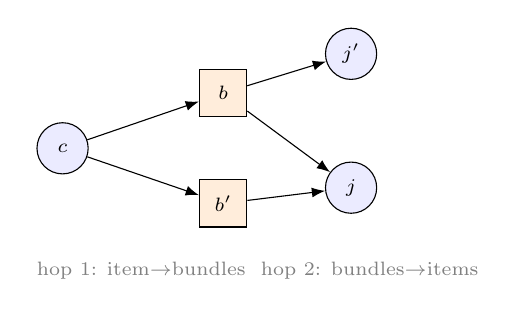
\begin{tikzpicture}[>=Latex,
  it/.style={circle,draw,fill=blue!8,minimum size=6.5mm,font=\scriptsize,inner sep=0pt},
  bu/.style={rectangle,draw,fill=orange!14,minimum size=6mm,font=\scriptsize,inner sep=1pt}]
\node[it](a){$c$};
\node[bu,right=14mm of a,yshift=7mm](b1){$b$};
\node[bu,right=14mm of a,yshift=-7mm](b2){$b'$};
\node[it,right=30mm of a,yshift=12mm](t2){$j'$};
\node[it,right=30mm of a,yshift=-5mm](t1){$j$};
\draw[->](a)--(b1);\draw[->](a)--(b2);
\draw[->](b1)--(t1);\draw[->](b2)--(t1);\draw[->](b1)--(t2);
\node[font=\scriptsize,gray] at (1.0,-1.55){hop 1: item$\to$bundles};
\node[font=\scriptsize,gray] at (3.9,-1.55){hop 2: bundles$\to$items};
\end{tikzpicture}
\end{center}
\captionof{figure}{\emph{One propagation step spreads a score two hops across the co-purchase graph.} Item $c$'s evidence flows
out to the bundles it belongs to and back down to \emph{their} other members $j,j'$ (both ends carrying the item
discount, the self-term subtracted). Applied to the pairwise score it yields the two-hop signal \code{diff2}; applied
to content vectors it builds the \code{bridge} (\S\ref{sec:content}). It is the factored product $B^{\!\top}(\cdots)B$,
never a dense $n\times n$ matrix---essential at $n=254{,}000$.}
\label{fig:prop}

% ======================================================================
\section{The signals, built one by one}
\label{sec:signals}

A \textbf{signal} is one scoring function $z_k(c\mid S)$: one opinion about each candidate. \textsc{BundleFuse}
computes about eleven of them, in three families. For each we give \emph{what it captures}, \emph{the exact
construction}, and \emph{which embedding (if any) it uses}. (Code: \code{score\_all\_signals},
\code{fullrank\_eval.py}:242--292.)

\subsection{Collaborative family (from $B$ only --- no embeddings)}

\begin{description}
\item[\code{cooc}] Raw co-occurrence $C\,\xs$ (\S\ref{sec:vocab}, Ex.~\ref{ex:cooc}). ``How often did it ship with
the seeds.''
\item[\code{ppmi}] Chance-corrected co-occurrence $\mathrm{PPMI}\,\xs$ (\S\ref{sec:pmi}, Ex.~\ref{ex:ppmi}).
``\dots more than chance would predict.''
\item[\code{csvd}] Similarity to the seeds' average collaborative fingerprint: with $U$ the PPMI-SVD embedding
(\S\ref{sec:svd}), score candidate $c$ by $\big\langle u_c,\ \tfrac1{|S|}\sum_{s\in S}u_s\big\rangle$. Captures
\emph{indirect} collaboration.
\item[\code{simp}] The degree-normalised pairwise score $W_{\text{pair}}\xs$ (\S\ref{sec:degnorm}) \emph{plus} a
higher-order ``incidence surplus'' $\Delta_{\text{inc}}$ described next.
\item[\code{diff2}] The two-hop propagated version of \code{simp} (\S\ref{sec:prop}): neighbours-of-neighbours.
\item[\code{pop}] Pure popularity, $\log(1+f_c)$, identical for every query. A backstop that knows nothing about $S$.
\end{description}

\paragraph{The higher-order incidence surplus $\Delta_{\text{inc}}$.} This is the one genuinely ``set-level''
collaborative term. Ordinary co-occurrence is \emph{pairwise}: it treats $S$ as a bag of seeds and sums seed-by-seed.
$\Delta_{\text{inc}}$ instead rewards a candidate for appearing in training bundles that already contain \emph{two or
more} of the current seeds together (\code{score\_simplicial\_incidence\_only}, \code{operators.py}:149--164):
\[
  \Delta_{\text{inc}}(c\mid S)=\sum_{b\ni c}(|b|+1)^{-0.5}\Big(\sum_{s\in b\cap S}(f_s+5)^{-0.5}\Big)\cdot\beta\cdot\max\!\big(0,\ |b\cap S|-1\big),
\]
with $\beta=1.5$. The factor $\max(0,|b\cap S|-1)$ is the crux: it is \textbf{zero unless a bundle overlaps the
seeds in at least two items}, so $\Delta_{\text{inc}}\equiv 0$ for single-seed queries ($|S|=1$) and whenever no
training bundle shares $\ge 2$ seeds with $S$. It is a surplus \emph{on top of} the pairwise term, not a replacement.
\emph{Honesty note: in our ablations this term moves Recall@20 by at most $+0.79$ points once the prior is in place;
it is near-inert, and we report that rather than overselling it.}

\paragraph{Second-order ``concordance'' $R_\gamma$ (Rao).} A second set-level term (signal \code{rao}) scores a
candidate by how strongly it is \emph{simultaneously} pulled by \emph{distinct, non-redundant} pairs of seeds, using
Rao's quadratic-entropy kernel to discount seeds that are near-duplicates of each other (same category / similar
embedding). With per-seed pulls $W_{\text{pair}}[\,\cdot,s]$ and a seed--seed redundancy kernel $K_S$,
\[
  R_\gamma(c\mid S)=\frac{\sum_{s\ne s'}K_S(s,s')\,W_{\text{pair}}[c,s]\,W_{\text{pair}}[c,s']}{\big(\sum_s W_{\text{pair}}[c,s]\big)+\tau},
\]
(\code{score\_rao\_concordance}, \code{operators.py}:179--217; $\tau=0.05$). The kernel $K_S$ is built from the
seeds' category labels \emph{and} their content embeddings, so this signal \emph{does} touch embeddings. Like
$\Delta_{\text{inc}}$ it is a small corrective, reported honestly as such.

\begin{center}
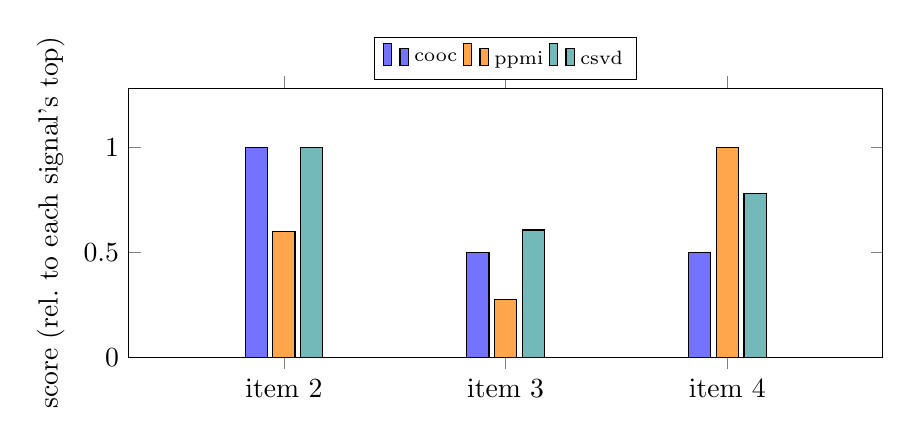
\begin{tikzpicture}
\begin{axis}[ybar,bar width=8pt,width=0.92\linewidth,height=5cm,
  symbolic x coords={item 2,item 3,item 4},xtick=data,
  ymin=0,ymax=1.28,enlarge x limits=0.35,
  ylabel={score (rel.\ to each signal's top)},
  legend style={font=\scriptsize,at={(0.5,1.03)},anchor=south,legend columns=3}]
\addplot[fill=blue!55]  coordinates {(item 2,1.0)(item 3,0.5)(item 4,0.5)};
\addplot[fill=orange!70]coordinates {(item 2,0.600)(item 3,0.275)(item 4,1.0)};
\addplot[fill=teal!55]  coordinates {(item 2,1.0)(item 3,0.606)(item 4,0.780)};
\legend{cooc,ppmi,csvd}
\end{axis}
\end{tikzpicture}
\end{center}
\captionof{figure}{\emph{Three collaborative opinions on $S=\{1\}$---and they disagree.} Bar heights are each signal's
score \emph{relative to its own top candidate} (raw values: \code{cooc}$=(2,1,1)$, \code{ppmi}$=(.34,.15,.56)$,
\code{csvd}$=(.90,.55,.70)$ over items $2,3,4$). Raw co-occurrence and the SVD fingerprint back the \emph{hub} item~$2$;
chance-corrected PPMI backs the \emph{rare-but-exclusive} item~$4$. This disagreement is exactly why fusion
(\S\ref{sec:fuse}) exists---no single collaborative signal is right everywhere.}
\label{fig:collabfam}

\subsection{Taxonomic family (from category/artist/album labels)}
\label{sec:tax}

These answer ``what \emph{kinds} of things go with these kinds of things,'' and crucially they work for \textbf{cold}
items (an unseen pair of jeans still has the category ``jeans'').

\begin{description}
\item[\code{cat}] \textbf{Category complementarity}, via PMI \emph{between categories}. Build a bundle$\times$category
count matrix $T_c$ (how many items of each category each bundle holds), form the category co-occurrence
$T_c^{\!\top}T_c$ (diagonal zeroed), and apply the \emph{same PPMI formula} as \S\ref{sec:pmi} but over categories,
giving $P_{\text{cat}}\in\R^{C\times C}$ (\code{operators.py}:262--269). Score a candidate by summing, over the
seeds' categories, the category-PMI into the candidate's category:
$\;\mathrm{cat}(c\mid S)=\sum_{s\in S}P_{\text{cat}}[\mathrm{cat}(s),\mathrm{cat}(c)]$. (``Shirts complement
trousers'' emerges as a large $P_{\text{cat}}$ entry.)
\item[\textit{slot self-exclusion}] A \emph{signed} correction added into \code{cat}: for a category that almost never
repeats inside a bundle (you rarely put two hats in one outfit), it \emph{subtracts} score from other items of that
same category, discouraging duplicate slots (\code{score\_slot\_saturation}, \code{operators.py}:307--316). The
threshold uses an empirical per-category duplication rate.
\item[\code{homo}] (music) \textbf{Homophily}: reward candidates by the same \emph{artist} or \emph{album} as the
seeds, with album weighted twice as much as artist (\code{fullrank\_eval.py}:273--275). Normalised by
$\sqrt{\text{degree}}$ so prolific artists do not swamp the score.
\item[\code{softcat}] (fashion) \textbf{Soft/fuzzy categories}: run $k$-means ($400$ clusters) on the multimodal
embedding, give each item a \emph{soft} assignment (a softmax of cosine-to-centroids), and apply the same PPMI
construction over the $400$ clusters. This captures sub-type complementarity finer than the official category labels.
\textbf{Uses embeddings} (for the clustering and soft assignment).
\end{description}

\begin{center}
\resizebox{\linewidth}{!}{%
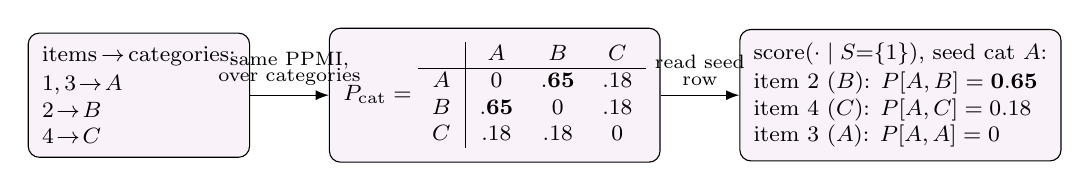
\begin{tikzpicture}[>=Latex,font=\footnotesize,
  bx/.style={draw,rounded corners,fill=violet!5,inner sep=5pt,align=left}]
\node[bx] (map) {items\,$\to$\,categories:\\[1pt] $1,3\!\to\!A$\\ $2\!\to\!B$\\ $4\!\to\!C$};
\node[bx,right=10mm of map] (P) {$P_{\text{cat}}=\begin{array}{c|ccc}&A&B&C\\\hline A&0&\mathbf{.65}&.18\\ B&\mathbf{.65}&0&.18\\ C&.18&.18&0\end{array}$};
\node[bx,right=10mm of P] (sc) {score$(\cdot\mid S{=}\{1\})$, seed cat $A$:\\[1pt] item $2$ ($B$): $P[A,B]=\mathbf{0.65}$\\ item $4$ ($C$): $P[A,C]=0.18$\\ item $3$ ($A$): $P[A,A]=0$};
\draw[->](map)--(P) node[midway,above,font=\scriptsize,align=center]{same PPMI,\\[-2pt]over categories};
\draw[->](P)--(sc) node[midway,above,font=\scriptsize,align=center]{read seed\\[-2pt]row};
\end{tikzpicture}}
\end{center}
\captionof{figure}{\emph{Taxonomic scoring: category-to-category PMI, machine-computed on toy categories.} Assign the
toy items categories $A,B,C$ as shown; the \emph{same} PPMI construction as Fig.~\ref{fig:build}, applied to the
bundle$\times$category counts, yields $P_{\text{cat}}$. For seed item~$1$ (category $A$) the candidate scores are just
row $A$: item~$2$ wins because ``$A$ complements $B$'' is a strong category pairing ($0.65$), item~$4$ gets a little
($0.18$), and same-category item~$3$ gets $0$. Crucially this needs \textbf{no co-occurrence of the candidate
itself}, so it scores cold items by \emph{what they are}.}
\label{fig:taxfam}

\subsection{Content family (from the embedding vectors)}
\label{sec:content}

This family is where the \S\ref{sec:emb} embeddings do their work. All three signals score a candidate by the cosine
similarity of its (processed) content vector to the \emph{average} content vector of the seeds:
$\mathrm{score}(c\mid S)=\big\langle \phi_c,\ \tfrac1{|S|}\sum_{s\in S}\phi_s\big\rangle$ for some processed feature
$\phi$ (\code{fullrank\_eval.py}:283--287). They differ in \emph{which} $\phi$:

\begin{description}
\item[\code{style} / \code{imgstyle} / \code{audiostyle}] \textbf{Category-disentangled} content. Raw embeddings are
dominated by ``what category is this'' (all boots look like boots), which is uninformative for \emph{within-outfit}
matching. \code{disentangle} (\code{operators.py}:323--330) subtracts the per-category mean embedding and
renormalises, leaving only the \emph{style} residual (``this boot's particular look''). Built separately for the
title embedding (\code{style}), the image embedding (\code{imgstyle}), and the audio embedding (\code{audiostyle}).
\item[\code{bridge}] \textbf{Graph-bridged} content. Take the disentangled style vectors and smooth them one hop over
the co-purchase graph (\S\ref{sec:prop}), then add that back: $\phi_{\text{bridge}}=\mathrm{normalise}(\text{style}+0.5\cdot
\mathcal{P}\,\text{style})$ (\code{build\_dense\_bridge}, \code{operators.py}:332--337). This lets content similarity
borrow a little collaborative structure---items that are both \emph{look-alike} and \emph{bought-with-alike} score
highest.
\item[\textit{(optional)} \code{contrast}] A tiny ($\le 0.30$M-parameter) set-attention encoder trained with a
contrastive loss. \textbf{It is off by default} (\code{ENCODER=0}); the whole point of the paper is that the
zero-parameter signals above are enough. When off, it contributes nothing.
\end{description}

\begin{center}
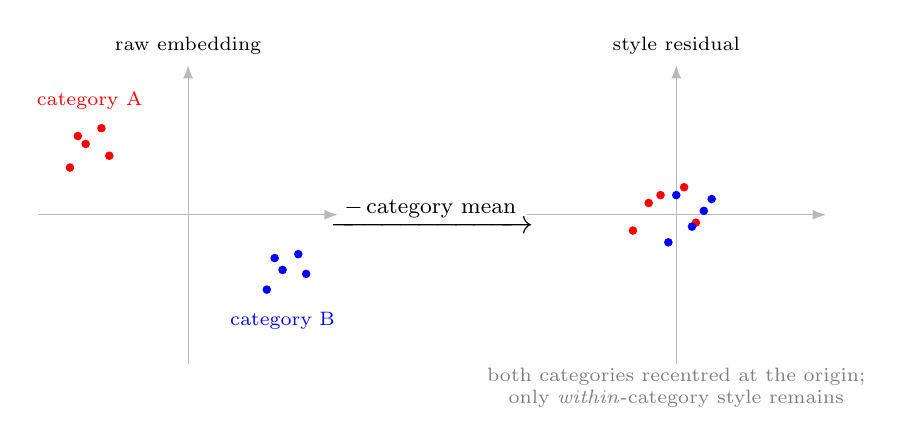
\begin{tikzpicture}[>=Latex,dot/.style={circle,fill,inner sep=1.1pt}]
 % left panel: raw embeddings
 \begin{scope}
   \draw[->,gray!55] (-1.9,0)--(1.9,0); \draw[->,gray!55] (0,-1.9)--(0,1.9);
   \node[font=\scriptsize] at (0,2.15) {raw embedding};
   \foreach \p in {(-1.3,0.9),(-1.5,0.6),(-1.1,1.1),(-1.4,1.0),(-1.0,0.75)} \node[dot,red] at \p {};
   \foreach \p in {(1.2,-0.7),(1.4,-0.5),(1.0,-0.95),(1.5,-0.75),(1.1,-0.55)} \node[dot,blue] at \p {};
   \node[font=\scriptsize,red]  at (-1.25,1.45) {category A};
   \node[font=\scriptsize,blue] at (1.2,-1.35)  {category B};
 \end{scope}
 % arrow
 \node at (3.1,0) {\large$\xrightarrow{\;-\,\text{category mean}\;}$};
 % right panel: disentangled
 \begin{scope}[xshift=6.2cm]
   \draw[->,gray!55] (-1.9,0)--(1.9,0); \draw[->,gray!55] (0,-1.9)--(0,1.9);
   \node[font=\scriptsize] at (0,2.15) {style residual};
   \foreach \p in {(-0.35,0.15),(-0.55,-0.2),(0.1,0.35),(-0.2,0.25),(0.25,-0.1)} \node[dot,red] at \p {};
   \foreach \p in {(0.2,-0.15),(0.45,0.2),(-0.1,-0.35),(0.35,0.05),(0.0,0.25)} \node[dot,blue] at \p {};
   \node[font=\scriptsize,align=center,gray] at (0,-2.2) {both categories recentred at the origin;\\only \emph{within}-category style remains};
 \end{scope}
\end{tikzpicture}
\end{center}
\captionof{figure}{\emph{What \code{disentangle} does.} Left: raw embeddings separate mostly by \emph{category} (all of A over
here, all of B over there)---useless for matching \emph{within} an outfit, since the seeds and the answer are
different categories by design. Subtracting each category's mean vector (right) cancels that bulk separation and
leaves only each item's \emph{style} deviation, which is what the content signals actually compare.}
\label{fig:disentangle}

\begin{center}
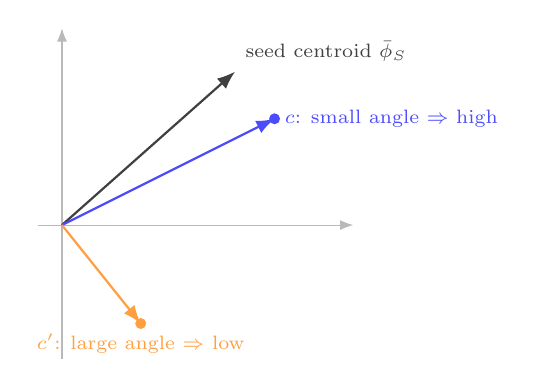
\begin{tikzpicture}[>=Latex,dot/.style={circle,fill,inner sep=1.4pt}]
\draw[->,gray!55](-0.3,0)--(3.7,0); \draw[->,gray!55](0,-1.7)--(0,2.5);
\draw[->,thick,black!75](0,0)--(2.2,1.95) node[above right,font=\scriptsize]{seed centroid $\bar\phi_S$};
\draw[->,thick,blue!70](0,0)--(2.7,1.35) node[dot]{} node[right,font=\scriptsize]{$c$: small angle $\Rightarrow$ high};
\draw[->,thick,orange!75](0,0)--(1.0,-1.25) node[dot]{} node[below,font=\scriptsize]{$c'$: large angle $\Rightarrow$ low};
\end{tikzpicture}
\end{center}
\captionof{figure}{\emph{Content scoring is cosine to the seeds' average style vector} (illustrative---the toy dataset
carries no embeddings). Each content signal (\code{style}/\code{imgstyle}/\code{bridge}) averages the seeds' processed
vectors into a centroid $\bar\phi_S$ and ranks candidates by $\langle\phi_c,\bar\phi_S\rangle$. Because the vectors are
category-disentangled (Fig.~\ref{fig:disentangle}), this rewards \emph{within-outfit style match}; like taxonomy it
uses no co-occurrence, so it too scores \textbf{cold} items.}
\label{fig:contentfam}

% ======================================================================
\section{From a signal to per-query numbers: scoring and standardising}
\label{sec:toscore}

Every signal above ultimately produces, for a batch of queries, a matrix $R_k\in\R^{n\times\text{nb}}$: one score per
(item, query). Collaborative signals get there by the ``$W\,\mathrm{Ind}$'' product (\S\ref{sec:vocab}); content and
\code{csvd} signals by the seed-centroid dot product (\S\ref{sec:content}).

\paragraph{Why we must standardise.} These raw scores live on wildly different scales---co-occurrence counts are
integers in $[0,\,\text{tens}]$, cosine similarities are in $[-1,1]$, PMI values are small positive logs. Adding them
directly would let whichever signal happens to have the biggest numbers dominate. So each signal is
\textbf{column-standardised} (\emph{per query}, across the $n$ candidates) to mean $0$, standard deviation $1$:
\begin{keybox}
\[
  z_k(c\mid S)=\frac{R_k(c\mid S)-\mathrm{mean}_{c'}R_k(c'\mid S)}{\mathrm{std}_{c'}R_k(c'\mid S)+10^{-9}} .
\]
\end{keybox}
(Code: \code{zcols}, \code{operators.py}:32--36.) After this, every signal speaks the same language---``how many
standard deviations above the field is this candidate, according to me''---and the weights in the next section are
comparing like with like.

% ======================================================================
\section{Fusion: four stages to the final score}
\label{sec:fuse}

Before the formulas, here is the whole machine on one page: the fixed inputs (left) feed the three signal families,
which are standardised and then combined into \emph{two} aggregates---a collaborative score $Y$ and a cold-start
prior $\mu_0$---that the final routing step mixes per candidate according to how often that candidate was seen.

\begin{center}
\resizebox{\linewidth}{!}{%
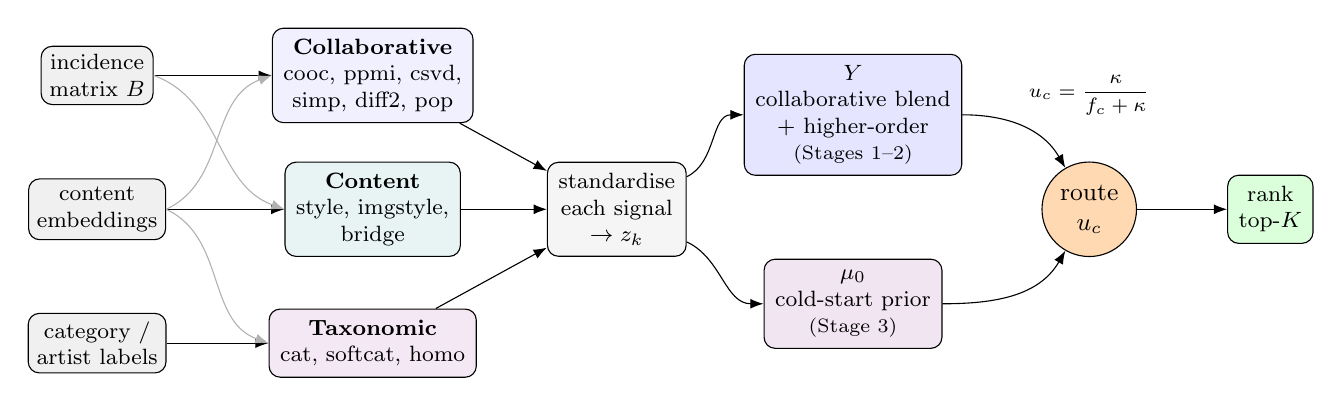
\begin{tikzpicture}[>=Latex,
 inp/.style={draw,rounded corners,fill=black!6,align=center,inner sep=3pt,font=\footnotesize},
 fam/.style={draw,rounded corners,align=center,inner sep=4pt,font=\footnotesize},
 agg/.style={draw,rounded corners,fill=blue!10,align=center,inner sep=4pt,font=\footnotesize},
 rnk/.style={draw,rounded corners,fill=green!14,align=center,inner sep=4pt,font=\footnotesize},
 rt/.style={draw,circle,fill=orange!30,inner sep=2pt,font=\small,align=center,minimum size=12mm}]
 % inputs
 \node[inp](B)  at (0,1.7)  {incidence\\matrix $B$};
 \node[inp](E)  at (0,0.0)  {content\\embeddings};
 \node[inp](L)  at (0,-1.7) {category /\\artist labels};
 % signal families
 \node[fam,fill=blue!6]  (col) at (3.5,1.7)  {\textbf{Collaborative}\\cooc, ppmi, csvd,\\simp, diff2, pop};
 \node[fam,fill=teal!9]  (con) at (3.5,0.0)  {\textbf{Content}\\style, imgstyle,\\bridge};
 \node[fam,fill=violet!9](tax) at (3.5,-1.7) {\textbf{Taxonomic}\\cat, softcat, homo};
 % standardise
 \node[fam,fill=black!4](z) at (6.6,0) {standardise\\each signal\\$\to z_k$};
 % aggregates
 \node[agg]              (Y)  at (9.6,1.2)  {$Y$\\collaborative blend\\$+$ higher-order\\{\scriptsize(Stages 1--2)}};
 \node[agg,fill=violet!10](mu) at (9.6,-1.2) {$\mu_0$\\cold-start prior\\{\scriptsize(Stage 3)}};
 % route + rank
 \node[rt] (u)   at (12.6,0) {route\\$u_c$};
 \node[rnk](out) at (14.9,0) {rank\\top-$K$};
 % main (solid) edges
 \draw[->](B)--(col); \draw[->](E)--(con); \draw[->](L)--(tax);
 % secondary (gray) edges
 \draw[->,gray!60](E.east) to[out=25,in=200] (col.west);
 \draw[->,gray!60](B.east) to[out=-20,in=160] (con.west);
 \draw[->,gray!60](E.east) to[out=-25,in=160] (tax.west);
 % families -> standardise
 \draw[->](col)--(z); \draw[->](con)--(z); \draw[->](tax)--(z);
 % standardise -> aggregates
 \draw[->](z) to[out=25,in=180] (Y.west);
 \draw[->](z) to[out=-25,in=180] (mu.west);
 % aggregates -> route -> rank
 \draw[->](Y) to[out=0,in=120] (u);
 \draw[->](mu) to[out=0,in=240] (u);
 \draw[->](u)--(out);
 \node[font=\scriptsize,align=center] at (12.6,1.45) {$u_c=\dfrac{\kappa}{f_c+\kappa}$};
\end{tikzpicture}}
\end{center}
\captionof{figure}{\emph{Solid arrows are each family's main input; gray arrows are secondary ones} (e.g.\ \code{bridge} also
reads $B$; \code{softcat} also reads embeddings). $f_c$ is the candidate's frequency, so cold candidates
($f_c\!=\!0$) route entirely to $\mu_0$. We now unpack the four stages.}
\label{fig:fusion}

Now we combine the standardised signals $\{z_k\}$ into one number per candidate. There are four stages; the only
quantities ``learned'' are a handful of scalars, each chosen by \textbf{greedy search on a validation split} to
maximise NDCG@20 (\code{fit\_simba}, \code{fullrank\_eval.py}:313--397). \S\ref{sec:selK} shows the result is
insensitive to \emph{which} cutoff we validate at, and why a cutoff-free objective would be worse.

\paragraph{Stage 1 --- weighted blend.} Pick a weight $w_k\ge 0$ per signal and form
\[
  Y_{\text{base}}(c\mid S)=\sum_k w_k\,z_k(c\mid S).
\]
The weights are found by \emph{greedy coordinate ascent}: sweep each $w_k$ over the grid
$\{0,0.25,0.5,1,1.5\}$, keep the change if validation NDCG@20 improves, repeat up to four passes
(\code{fullrank\_eval.py}:340--354). A signal that never helps simply gets weight $0$---the method prunes itself.
Afterwards a backward-elimination pass tries to \emph{drop} optional signals (bridge, contrast, softcat, homo) if
doing so does not hurt validation (\code{prune\_weights\_val}).

\paragraph{Stage 2 --- fold in the set-level terms.} Blend the pairwise base with its incidence-augmented version and
the Rao term, via two more validation-picked scalars $\alpha\in\{0,0.5,1\}$ and $\gamma\in\{0,0.2,0.35\}$:
\[
  Y(c\mid S)=(1-\alpha)\,Y_{\text{base}}^{\text{pair}}+\alpha\,Y_{\text{base}}^{\text{inc}}+\gamma\,z_{\text{rao}}.
\]
Here $Y_{\text{base}}^{\text{pair}}$ uses the \emph{purely pairwise} versions of \code{simp}/\code{diff2} and
$Y_{\text{base}}^{\text{inc}}$ uses the \emph{incidence-augmented} ones, so $\alpha$ literally dials how much of the
higher-order surplus to admit. (On most datasets $\alpha,\gamma$ come out small---the honest ``near-inert'' finding.)

\paragraph{Stage 3 --- the cold-start prior $\mu_0$.} Build a \emph{second} score that needs no collaborative
exposure of the candidate, from the metadata/content signals only:
\[
  \mu_0(c\mid S)=\text{(frozen scale)}\times\Big(\sum_{k\in\text{prior keys}}w_k\,z_k+\gamma\,z_{\text{rao}}\ [+\,w_{\text{pop}}z_{\text{pop}}]\Big),
\]
where ``prior keys'' are the taxonomic/content signals that earned positive weight (\code{cat}, \code{softcat},
\code{style}, \code{imgstyle}, \code{bridge} for fashion; \code{cat}, \code{homo}, \code{audiostyle}, \code{bridge}
for music). The ``frozen scale'' is a single number $=\mathrm{std}(Y)/\mathrm{std}(\text{raw prior})$ computed
\textbf{on the validation set and then frozen}, so that at test time $\mu_0$ is on the same scale as $Y$ and---
critically---\emph{a candidate's score never depends on which other queries happen to be in its test batch}
(\code{fullrank\_eval.py}:380--385). This is why the method is exactly reproducible.

\paragraph{Stage 4 --- frequency-confidence routing (shrinkage).} Combine the collaborative blend $Y$ and the prior
$\mu_0$ per candidate, trusting $Y$ more when the candidate is \emph{frequent} and $\mu_0$ more when it is
\emph{rare}:
\begin{keybox}
\[
  \hat\theta(c\mid S)=(1-u_c)\,Y(c\mid S)+u_c\,\mu_0(c\mid S),\qquad u_c=\frac{\kappa}{f_c+\kappa}.
\]
\end{keybox}
The single dial $\kappa\ge 0$ is picked on validation (\code{conjugate\_posterior}, \code{operators.py}:526--543).
Read the two extremes:
\begin{itemize}
\item \textbf{Cold candidate}, $f_c=0\Rightarrow u_c=1\Rightarrow\hat\theta=\mu_0$: ranked purely by taxonomy/content,
since it has no co-occurrence evidence at all.
\item \textbf{Very frequent candidate}, $f_c\gg\kappa\Rightarrow u_c\to 0\Rightarrow\hat\theta\to Y$: ranked by the
collaborative evidence, which for a hub is plentiful and trustworthy.
\end{itemize}

\begin{center}
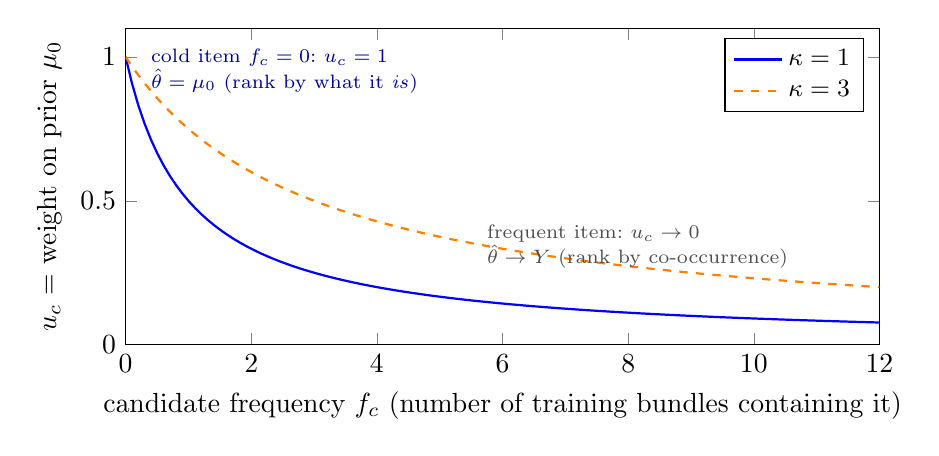
\begin{tikzpicture}
\begin{axis}[width=0.92\linewidth,height=5.6cm,
  xlabel={candidate frequency $f_c$ (number of training bundles containing it)},
  ylabel={$u_c$ = weight on prior $\mu_0$},
  domain=0:12,samples=120,ymin=0,ymax=1.1,xmin=0,xmax=12,xtick={0,2,4,6,8,10,12},
  legend style={font=\small,at={(0.98,0.97)},anchor=north east}]
\addplot[thick,blue]{1/(x+1)};
\addplot[thick,orange,dashed]{3/(x+3)};
\legend{$\kappa=1$,$\kappa=3$}
\node[anchor=north west,font=\scriptsize,align=left,text=blue!60!black]
  at (axis cs:0.25,1.06) {cold item $f_c=0$:\ $u_c=1$\\$\hat\theta=\mu_0$ (rank by what it \emph{is})};
\node[anchor=west,font=\scriptsize,align=left,text=black!70]
  at (axis cs:5.6,0.34) {frequent item:\ $u_c\to 0$\\$\hat\theta\to Y$ (rank by co-occurrence)};
\end{axis}
\end{tikzpicture}
\end{center}
\captionof{figure}{\emph{The routing dial.} As a candidate is seen more often, weight slides off the prior and onto the
collaborative evidence. The single learned scalar $\kappa$ sets \emph{how fast}: larger $\kappa$ (orange) keeps
trusting the prior up to higher frequencies. It is chosen on validation, not derived from a model.
The \emph{form} of this rule is the posterior mean of a Normal--Normal model (derived in \code{formalization.tex});
but we do \emph{not} estimate $\kappa$ from that model---it is just selected on validation---so in practice Stage 4 is
a principled, frequency-aware interpolation between ``what co-occurrence says'' and ``what the item \emph{is}.''
Finally we rank $\I\setminus S$ by $\hat\theta(\cdot\mid S)$ and return the top $K$.}
\label{fig:shrink}

\begin{example}[the four stages on one query]
Take $S=\{1\}$ on the toy data and suppose validation selected weights $w_{\text{ppmi}}=1$, $w_{\text{cat}}=0.5$
(all else $0$), $\alpha=\gamma=0$, and $\kappa=1$. From Example~\ref{ex:ppmi} the \code{ppmi} raw column is
$(0,0.336,0.154,0.560)$; standardising (Stage 0) and blending (Stage 1) gives $Y$. Suppose the category prior
$\mu_0$ (Stage 3) favours item $2$ (a complementary category to item $1$). Item $4$ is rare ($f_4=1$) so
$u_4=\tfrac{1}{1+1}=0.5$: its final score is the \emph{average} of its strong collaborative evidence and the prior.
Item $2$ is frequent ($f_2=3$) so $u_2=\tfrac{1}{4}=0.25$: it leans $75\%$ on collaboration. The routing thus lets
the rare-but-exclusive item $4$ keep most of its PPMI boost while a cold item (if any) would fall back entirely on
the category prior. Every number here is a fixed function of $S$---no randomness, no test-batch dependence.
\end{example}

\begin{center}
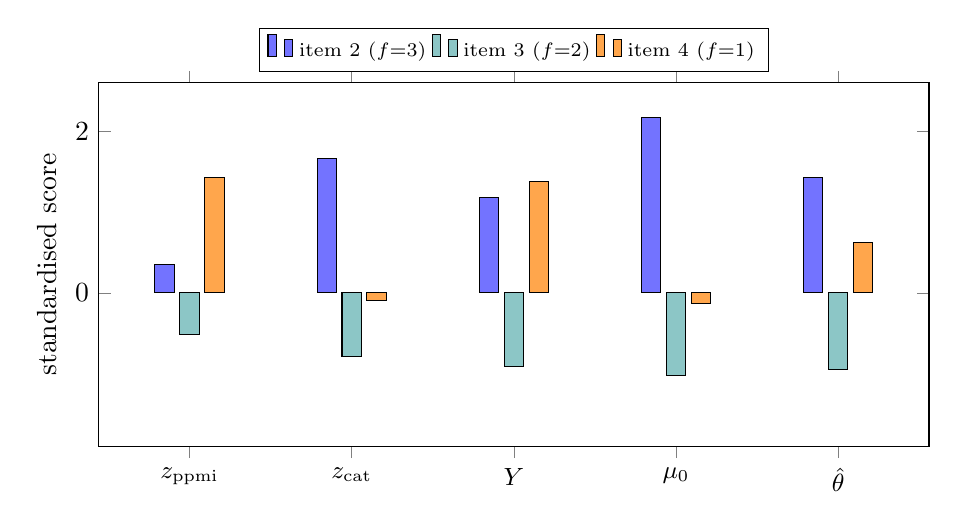
\begin{tikzpicture}
\begin{axis}[ybar,bar width=7pt,width=\linewidth,height=6.2cm,
  symbolic x coords={$z_{\mathrm{ppmi}}$,$z_{\mathrm{cat}}$,$Y$,$\mu_0$,$\hat\theta$},
  xtick=data,x tick label style={font=\small},
  ymin=-1.9,ymax=2.6,enlarge x limits=0.14,
  ylabel={standardised score},
  legend style={font=\scriptsize,at={(0.5,1.03)},anchor=south,legend columns=3}]
\addplot[fill=blue!55]  coordinates {($z_{\mathrm{ppmi}}$,0.352)($z_{\mathrm{cat}}$,1.663)($Y$,1.183)($\mu_0$,2.174)($\hat\theta$,1.431)};
\addplot[fill=teal!45]  coordinates {($z_{\mathrm{ppmi}}$,-0.519)($z_{\mathrm{cat}}$,-0.782)($Y$,-0.910)($\mu_0$,-1.022)($\hat\theta$,-0.948)};
\addplot[fill=orange!70]coordinates {($z_{\mathrm{ppmi}}$,1.424)($z_{\mathrm{cat}}$,-0.099)($Y$,1.375)($\mu_0$,-0.129)($\hat\theta$,0.623)};
\legend{item 2 ($f{=}3$),item 3 ($f{=}2$),item 4 ($f{=}1$)}
\end{axis}
\end{tikzpicture}
\end{center}
\captionof{figure}{\emph{The four stages on $S=\{1\}$, every bar machine-computed} (weights $w_{\mathrm{ppmi}}{=}1$,
$w_{\mathrm{cat}}{=}0.5$, $\alpha{=}\gamma{=}0$, $\kappa{=}1$). Left to right: the two example signals, then the
collaborative blend $Y$ (Stages 1--2), the cold-start prior $\mu_0$ (Stage 3), and the routed final $\hat\theta$
(Stage 4). Follow item~$4$ (orange): PPMI loves it ($1.42$) and it
stays high in the collaborative blend $Y$ ($1.38$), but the category prior $\mu_0$ is \emph{cold} on it ($-0.13$).
Because item~$4$ is rare ($f{=}1\Rightarrow u_c{=}0.5$), routing (Stage 4) pulls its final score halfway to that low
prior, down to $\hat\theta{=}0.62$. Item~$2$ (blue) is backed by \emph{both} $Y$ and $\mu_0$ and is frequent
($u_c{=}0.25$), so it stays on top. Final ranking $\mathbf{2\succ4\succ3}$; the seed~$1$ is masked. This is the whole
machine turning one partial bundle into one ordered completion.}
\label{fig:stages}

% ======================================================================
\subsection{Why validate at NDCG@20 --- and why not a ``cutoff-free'' loss}
\label{sec:selK}

A fair question: if we \emph{select} the weights on NDCG@20 and also \emph{report} at cutoff $20$, are we not
just tuning to the number we are graded on? The honest answer has two parts, both measured
(\code{results/selection\_sensitivity.md}).

\paragraph{The result does not depend on the cutoff.} Re-selecting the weights at NDCG@$K$ for
$K\in\{10,20,50,100\}$ and re-measuring test Recall@20 gives \emph{the same answer} across a tenfold range of
cutoffs --- a flat plateau (below). Selecting \emph{directly} on Recall@20 is no better (electronic
$0.486$ vs.\ NDCG@20's $0.514$). So $K=20$ is not cherry-picked, and NDCG@20 is not ``optimising the reported
metric'' --- it is a smoother, better-conditioned surrogate at the same \emph{operating point}.

\begin{center}
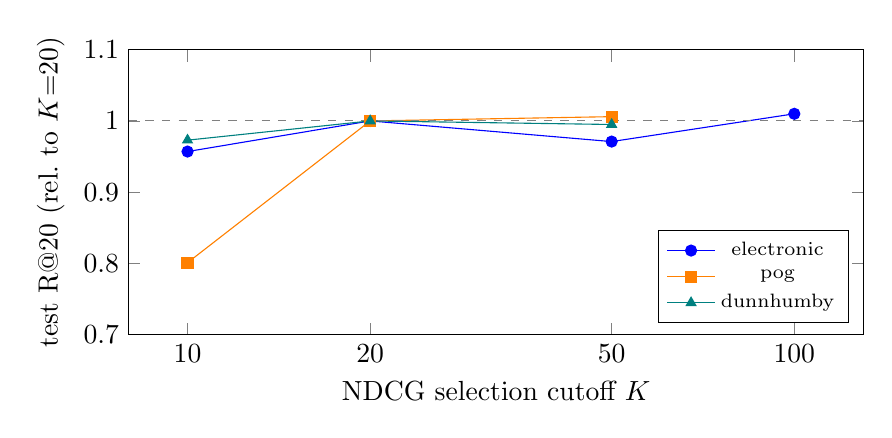
\begin{tikzpicture}
\begin{axis}[width=0.9\linewidth,height=5.2cm,xmode=log,log basis x=10,
  xtick={10,20,50,100},xticklabels={10,20,50,100},
  xlabel={NDCG selection cutoff $K$}, ylabel={test R@20 (rel.\ to $K{=}20$)},
  ymin=0.7,ymax=1.1,xmin=8,xmax=130,
  legend style={font=\scriptsize,at={(0.98,0.04)},anchor=south east}]
\addplot[mark=*,blue]        coordinates {(10,0.957)(20,1.0)(50,0.971)(100,1.010)};
\addplot[mark=square*,orange] coordinates {(10,0.801)(20,1.0)(50,1.006)};
\addplot[mark=triangle*,teal] coordinates {(10,0.973)(20,1.0)(50,0.995)};
\draw[dashed,gray] (axis cs:8,1.0)--(axis cs:130,1.0);
\legend{electronic,pog,dunnhumby}
\end{axis}
\end{tikzpicture}
\end{center}
\captionof{figure}{\emph{Flat plateau.} Test Recall@20 (normalised to the $K{=}20$ run) is essentially unchanged whether
weights are selected at NDCG@10, 20, 50 or 100. Cutoff-free objectives, by contrast, land anywhere from
$0.03\times$ to $0.94\times$ depending on the dataset (table below).}
\label{fig:plateau}

\paragraph{A cutoff-free objective is worse, and unreliably so.} The tempting ``generic'' alternatives all
under-perform because they do not target the retrieval region a short recommendation slate actually uses:

\begin{center}\small
\begin{tabular}{@{}l r r r@{}}
\toprule
selection objective & electronic & pog & dunnhumby \\
\midrule
\textbf{NDCG@20} (used) & \textbf{0.514} & \textbf{0.064} & \textbf{0.151} \\
Recall@20 (ERM on reported metric) & 0.486 & 0.066 & 0.148 \\
MRR ($1/\text{rank}$, cutoff-free) & 0.327 & \textbf{0.002} & 0.142 \\
softmax NLL (cutoff-free, proper score) & 0.452 & 0.044 & 0.140 \\
\bottomrule
\end{tabular}
\end{center}

\noindent MRR weights rank-$1$ so heavily that moving a true item from rank $25$ to $18$ --- exactly what
Recall@20 rewards --- barely registers; it is fine on dense collaborative data (dunnhumby) but
\emph{catastrophic} on sparse content data (pog, $0.002$). The softmax NLL is a proper scoring rule for the
\emph{whole} score distribution, so it spends effort on calibration far below the slate and is consistently
$\sim$7--31\% below NDCG@20. \textbf{The lesson is the opposite of ``do not tune to their metric'': you should
select at the operating point you deploy at} (a short slate), the exact cutoff inside a broad band does not
matter, and no cutoff-free loss improves on it.

% ======================================================================
\section{The ledger: what is learned vs.\ fixed}
\label{sec:ledger}

\begin{center}\small
\begin{tabular}{@{}p{0.34\linewidth} p{0.60\linewidth}@{}}
\toprule
\textbf{Fixed inputs (not learned)} & embeddings (\S\ref{sec:emb}, shipped with the dataset); category/artist/album
labels; the bundle incidence matrix $B$. \\[2pt]
\textbf{Deterministic constructions} & $C$, PPMI, PPMI-SVD fingerprints, $W_{\text{pair}}$, category/soft-cluster
PMI, disentangled + bridged content. All closed-form functions of the fixed inputs---\emph{zero trainable
parameters}. \\[2pt]
\textbf{Selected on validation (the only ``learning'')} & the per-signal weights $w_k$ (grid
$\{0,0.25,0.5,1,1.5\}$); the higher-order mixers $\alpha,\gamma$; the shrinkage dial $\kappa$; the prior scale
(computed, then frozen). A few dozen scalar choices total, by grid search---no gradients, no neural weights. \\[2pt]
\textbf{Off by default} & the $\le 0.30$M-parameter contrastive set-encoder (\code{ENCODER=0}). \\
\bottomrule
\end{tabular}
\end{center}

\begin{keybox}
\textbf{In one paragraph.} \textsc{BundleFuse} turns the bundle incidence matrix and a set of fixed content
embeddings into about eleven standardised ``opinions'' per candidate---raw and chance-corrected co-occurrence, a
co-occurrence SVD fingerprint, size-aware pairwise and two-hop scores, two small set-level corrections, category and
soft-category complementarity PMIs, metadata homophily, and category-disentangled / graph-bridged content
similarity. It blends them with validation-picked weights into a collaborative score $Y$ and a cold-start prior
$\mu_0$, then routes the two per candidate by $\hat\theta=(1-u_c)Y+u_c\mu_0$ with $u_c=\kappa/(f_c+\kappa)$, so
frequent items are judged by co-occurrence and rare/cold items by what they \emph{are}. The scoring core trains
nothing; the embeddings are inputs, and the handful of dials are chosen by grid search on held-out bundles.
\end{keybox}

\end{document}
